\vspace{0.5em}\noindent\textbf{Week 8 - End-to-End Deployment and Operational
Validation}\par

\vspace{0.5em}\noindent\textbf{Objectives}\par

During Week 8, I finalized the production deployment path for the
Internship Application Tracker. I built and validated the deployment
model for Amazon EKS workloads, Application Load Balancer routing, S3
and CloudFront frontend delivery, AWS-managed data services,
event-driven processing, and cost tracking.

I used the Week 08 AWS evidence directory as the source of truth for
this section. The cost figures come from the July 1-28, 2026 AWS cost
summary, the Billing credits screenshot, and the Cost Explorer overview
screenshot. The finalized monthly bill and the AWS Pricing Calculator
estimate are still unavailable.

\vspace{0.5em}\noindent\textbf{Tasks Completed}\par

{
\begingroup
\small
\setlength{\tabcolsep}{3pt}
\renewcommand{\arraystretch}{1.15}
\begin{longtable}{@{}
  >{\raggedright\arraybackslash}p{(\linewidth - 4\tabcolsep) * \real{0.3333}}
  >{\raggedright\arraybackslash}p{(\linewidth - 4\tabcolsep) * \real{0.3333}}
  >{\raggedright\arraybackslash}p{(\linewidth - 4\tabcolsep) * \real{0.3333}}@{}}
\toprule\noalign{}
\begin{minipage}[b]{\linewidth}\raggedright
Status
\end{minipage} & \begin{minipage}[b]{\linewidth}\raggedright
Task
\end{minipage} & \begin{minipage}[b]{\linewidth}\raggedright
Evidence basis
\end{minipage} \\
\midrule\noalign{}
\endhead
\bottomrule\noalign{}
\endlastfoot
Completed & Added the SageMaker-oriented AI service integration and
deployment path while preserving worker-facing routes. & Source
references from the project implementation and
\texttt{sagemaker-\allowbreak{}health.\allowbreak{}png}. \\
Completed & Fixed deploy-app image propagation and deterministic ECR
image selection. & Source references from the CI/CD workflow
implementation. \\
Completed & Removed frontend Kubernetes resources from the current
runtime path so frontend delivery uses S3 and CloudFront instead of an
EKS frontend pod. & Source references from the deployment scripts and
architecture notes. \\
Completed & Verified Amazon RDS PostgreSQL and Amazon ElastiCache Valkey
runtime status from AWS CLI screenshots. & \texttt{RDS-\allowbreak{}health.\allowbreak{}png},
\texttt{REDIS-\allowbreak{}health.\allowbreak{}png}. \\
Completed & Verified the SageMaker endpoint runtime status from AWS CLI
screenshot evidence. & \texttt{sagemaker-\allowbreak{}health.\allowbreak{}png}. \\
Partially completed & Verified EKS workloads and ALB runtime state from
AWS CLI screenshots. & EKS workloads were running, but the ALB target
health screenshot showed mixed unhealthy targets. \\
Completed & Added CloudFront, S3, DynamoDB, and SQS runtime evidence. &
Sanitized screenshots: \texttt{Cloudfront-\allowbreak{}evidence.\allowbreak{}png},
\texttt{S3-\allowbreak{}evidenc.\allowbreak{}png}, \texttt{DynamoDB-\allowbreak{}evidenc.\allowbreak{}png},
\texttt{SQS-\allowbreak{}evidence.\allowbreak{}png}. \\
Partially completed & Added AWS cost evidence for July 1-28, 2026. &
July cost summary, \texttt{total-\allowbreak{}cost-\allowbreak{}july.\allowbreak{}png}, and
\texttt{Cost-\allowbreak{}evidence.\allowbreak{}png}; Pricing Calculator remains blocked. \\
\end{longtable}
\endgroup
}

\vspace{0.5em}\noindent\textbf{Technical Implementation}\par

The final deployment model separates static frontend hosting from
long-running service workloads. Backend, chat, worker, and AI services
run on EKS. Static browser assets are intended to be served through S3
and CloudFront, while API, chat, and Socket.IO paths route through the
ALB.

\{\{\textless{} mermaid \textgreater\}\} graph LR Browser{[}``User
browser''{]} --\textgreater{} CF{[}``CloudFront distribution''{]} CF
--\textgreater{} S3{[}``S3 frontend bucket''{]} CF --\textgreater{}
ALB{[}``ALB for /api, /chat, /socket.io''{]} ALB --\textgreater{}
Backend{[}``EKS backend''{]} ALB --\textgreater{} Chat{[}``EKS
chat-service''{]} Backend --\textgreater{} RDS{[}``RDS PostgreSQL''{]}
Chat --\textgreater{} Redis{[}``ElastiCache Valkey''{]} Chat
--\textgreater{} DDB{[}``DynamoDB chat tables''{]} Backend
--\textgreater{} Worker{[}``processing worker''{]} Worker
--\textgreater{} AI{[}``ai-service''{]} AI --\textgreater{}
SageMaker{[}``SageMaker endpoint''{]} Backend --\textgreater{}
Outbox{[}``outbox dispatcher''{]} Outbox --\textgreater{} SQS{[}``SQS
queue''{]} SQS --\textgreater{} Lambda{[}``Lambda notification
handler''{]} \{\{\textless{} /mermaid \textgreater\}\}

The CI/CD workflow supports deployment modes including
\texttt{validate}, \texttt{deploy-\allowbreak{}app}, \texttt{deploy-\allowbreak{}public},
\texttt{deploy-\allowbreak{}frontend}, \texttt{rollout}, and \texttt{full}. Backend,
chat, and AI images are tagged with the GitHub commit SHA. The frontend
deployment path builds the Vite app, publishes static files to S3, and
invalidates CloudFront when frontend deployment is enabled.

\vspace{0.5em}\noindent\textbf{AWS Runtime Evidence}\par

The runtime evidence below uses only files that I placed in the Week 08
AWS evidence directory. I reviewed the following files:

\begin{itemize}
\tightlist
\item
  \texttt{ALB-\allowbreak{}target-\allowbreak{}health.\allowbreak{}png}
\item
  \texttt{ALB-\allowbreak{}target.\allowbreak{}png}
\item
  \texttt{Cloudfront-\allowbreak{}evidence.\allowbreak{}png}
\item
  \texttt{Cost-\allowbreak{}evidence.\allowbreak{}png}
\item
  \texttt{DynamoDB-\allowbreak{}evidenc.\allowbreak{}png}
\item
  \texttt{eks-\allowbreak{}deployment-\allowbreak{}rollout-\allowbreak{}success.\allowbreak{}png}
\item
  \texttt{eks-\allowbreak{}runtime-\allowbreak{}pods-\allowbreak{}2026-\allowbreak{}07-\allowbreak{}28.\allowbreak{}png}
\item
  \texttt{lambda.\allowbreak{}png}
\item
  \texttt{Lambda-\allowbreak{}evidence.\allowbreak{}png}
\item
  \texttt{lambda-\allowbreak{}cloudwatch-\allowbreak{}evidence.\allowbreak{}png}
\item
  \texttt{RDS-\allowbreak{}health.\allowbreak{}png}
\item
  \texttt{REDIS-\allowbreak{}health.\allowbreak{}png}
\item
  \texttt{S3-\allowbreak{}evidenc.\allowbreak{}png}
\item
  \texttt{sagemaker-\allowbreak{}health.\allowbreak{}png}
\item
  \texttt{SQS-\allowbreak{}evidence.\allowbreak{}png}
\item
  \texttt{total-\allowbreak{}cost-\allowbreak{}july.\allowbreak{}png}
\end{itemize}

I did not find \texttt{.\allowbreak{}txt}, \texttt{.\allowbreak{}log}, \texttt{.\allowbreak{}json},
\texttt{.\allowbreak{}yaml}, or \texttt{.\allowbreak{}yml} evidence files in this directory, so I
did not include long CLI log excerpts.

\vspace{0.5em}\noindent\textbf{Runtime Evidence Summary}\par

{
\begingroup
\small
\setlength{\tabcolsep}{3pt}
\renewcommand{\arraystretch}{1.15}
\begin{longtable}{@{}
  >{\raggedright\arraybackslash}p{(\linewidth - 6\tabcolsep) * \real{0.2500}}
  >{\raggedright\arraybackslash}p{(\linewidth - 6\tabcolsep) * \real{0.2500}}
  >{\raggedright\arraybackslash}p{(\linewidth - 6\tabcolsep) * \real{0.2500}}
  >{\raggedright\arraybackslash}p{(\linewidth - 6\tabcolsep) * \real{0.2500}}@{}}
\toprule\noalign{}
\begin{minipage}[b]{\linewidth}\raggedright
AWS service
\end{minipage} & \begin{minipage}[b]{\linewidth}\raggedright
Evidence status
\end{minipage} & \begin{minipage}[b]{\linewidth}\raggedright
Runtime status
\end{minipage} & \begin{minipage}[b]{\linewidth}\raggedright
Evidence
\end{minipage} \\
\midrule\noalign{}
\endhead
\bottomrule\noalign{}
\endlastfoot
Amazon EKS & Available & Partially verified: nodes, pods, jobs, and
deployments were healthy; cluster \texttt{ACTIVE} status was not
directly captured & \texttt{eks-\allowbreak{}runtime-\allowbreak{}pods-\allowbreak{}2026-\allowbreak{}07-\allowbreak{}28.\allowbreak{}png},
\texttt{eks-\allowbreak{}deployment-\allowbreak{}rollout-\allowbreak{}success.\allowbreak{}png} \\
Application Load Balancer & Available & Partially operational: load
balancer was active and target groups existed, but target health was
mixed and included unhealthy targets & \texttt{ALB-\allowbreak{}target-\allowbreak{}health.\allowbreak{}png},
\texttt{ALB-\allowbreak{}target.\allowbreak{}png} \\
Amazon CloudFront & Available & Partially verified: I captured
monitoring metrics for requests, data transfer, and distribution error
rates & \texttt{Cloudfront-\allowbreak{}evidence.\allowbreak{}png} \\
Amazon S3 & Available & Verified frontend bucket objects after
account-suffix redaction & \texttt{S3-\allowbreak{}evidenc.\allowbreak{}png} \\
Amazon RDS & Available & Available & \texttt{RDS-\allowbreak{}health.\allowbreak{}png} \\
Amazon ElastiCache & Available & Available &
\texttt{REDIS-\allowbreak{}health.\allowbreak{}png} \\
Amazon DynamoDB & Available & Verified: chat tables and Lambda dedupe
table are Active and on-demand & \texttt{DynamoDB-\allowbreak{}evidenc.\allowbreak{}png} \\
Amazon SQS & Available & Verified: main queue and DLQ exist, show zero
visible/in-flight messages, and use SSE-SQS &
\texttt{SQS-\allowbreak{}evidence.\allowbreak{}png} \\
AWS Lambda & Available & Partially verified: function configuration,
source view, and CloudWatch log group exist; invocation result still not
verified & \texttt{lambda.\allowbreak{}png}, \texttt{Lambda-\allowbreak{}evidence.\allowbreak{}png},
\texttt{lambda-\allowbreak{}cloudwatch-\allowbreak{}evidence.\allowbreak{}png} \\
Amazon SageMaker & Available & InService &
\texttt{sagemaker-\allowbreak{}health.\allowbreak{}png} \\
\end{longtable}
\endgroup
}

\vspace{0.5em}\noindent\textbf{Amazon EKS}\par

\textbf{Evidence status:} Available \textbf{Runtime status:} Partially
verified

I verified two Ready worker nodes, running application pods, completed
migration/init jobs, and ready deployments in the \texttt{internship}
namespace. The visible workloads include \texttt{ai-\allowbreak{}service},
\texttt{backend}, \texttt{backend-\allowbreak{}outbox-\allowbreak{}dispatcher},
\texttt{backend-\allowbreak{}processing-\allowbreak{}worker}, and \texttt{chat-\allowbreak{}service}.

The same evidence confirms deployment readiness:

\begin{itemize}
\tightlist
\item
  \texttt{ai-\allowbreak{}service}: 1/1 ready
\item
  \texttt{backend}: 2/2 ready
\item
  \texttt{backend-\allowbreak{}outbox-\allowbreak{}dispatcher}: 1/1 ready
\item
  \texttt{backend-\allowbreak{}processing-\allowbreak{}worker}: 1/1 ready
\item
  \texttt{chat-\allowbreak{}service}: 2/2 ready
\end{itemize}

I did not capture an \texttt{aws\ eks\ describe-\allowbreak{}cluster} output showing
the EKS cluster status as \texttt{ACTIVE}. For that reason, I classify
EKS as partially verified instead of claiming that full cluster-level
evidence was captured.

\begin{figure}
\centering
\pandocbounded{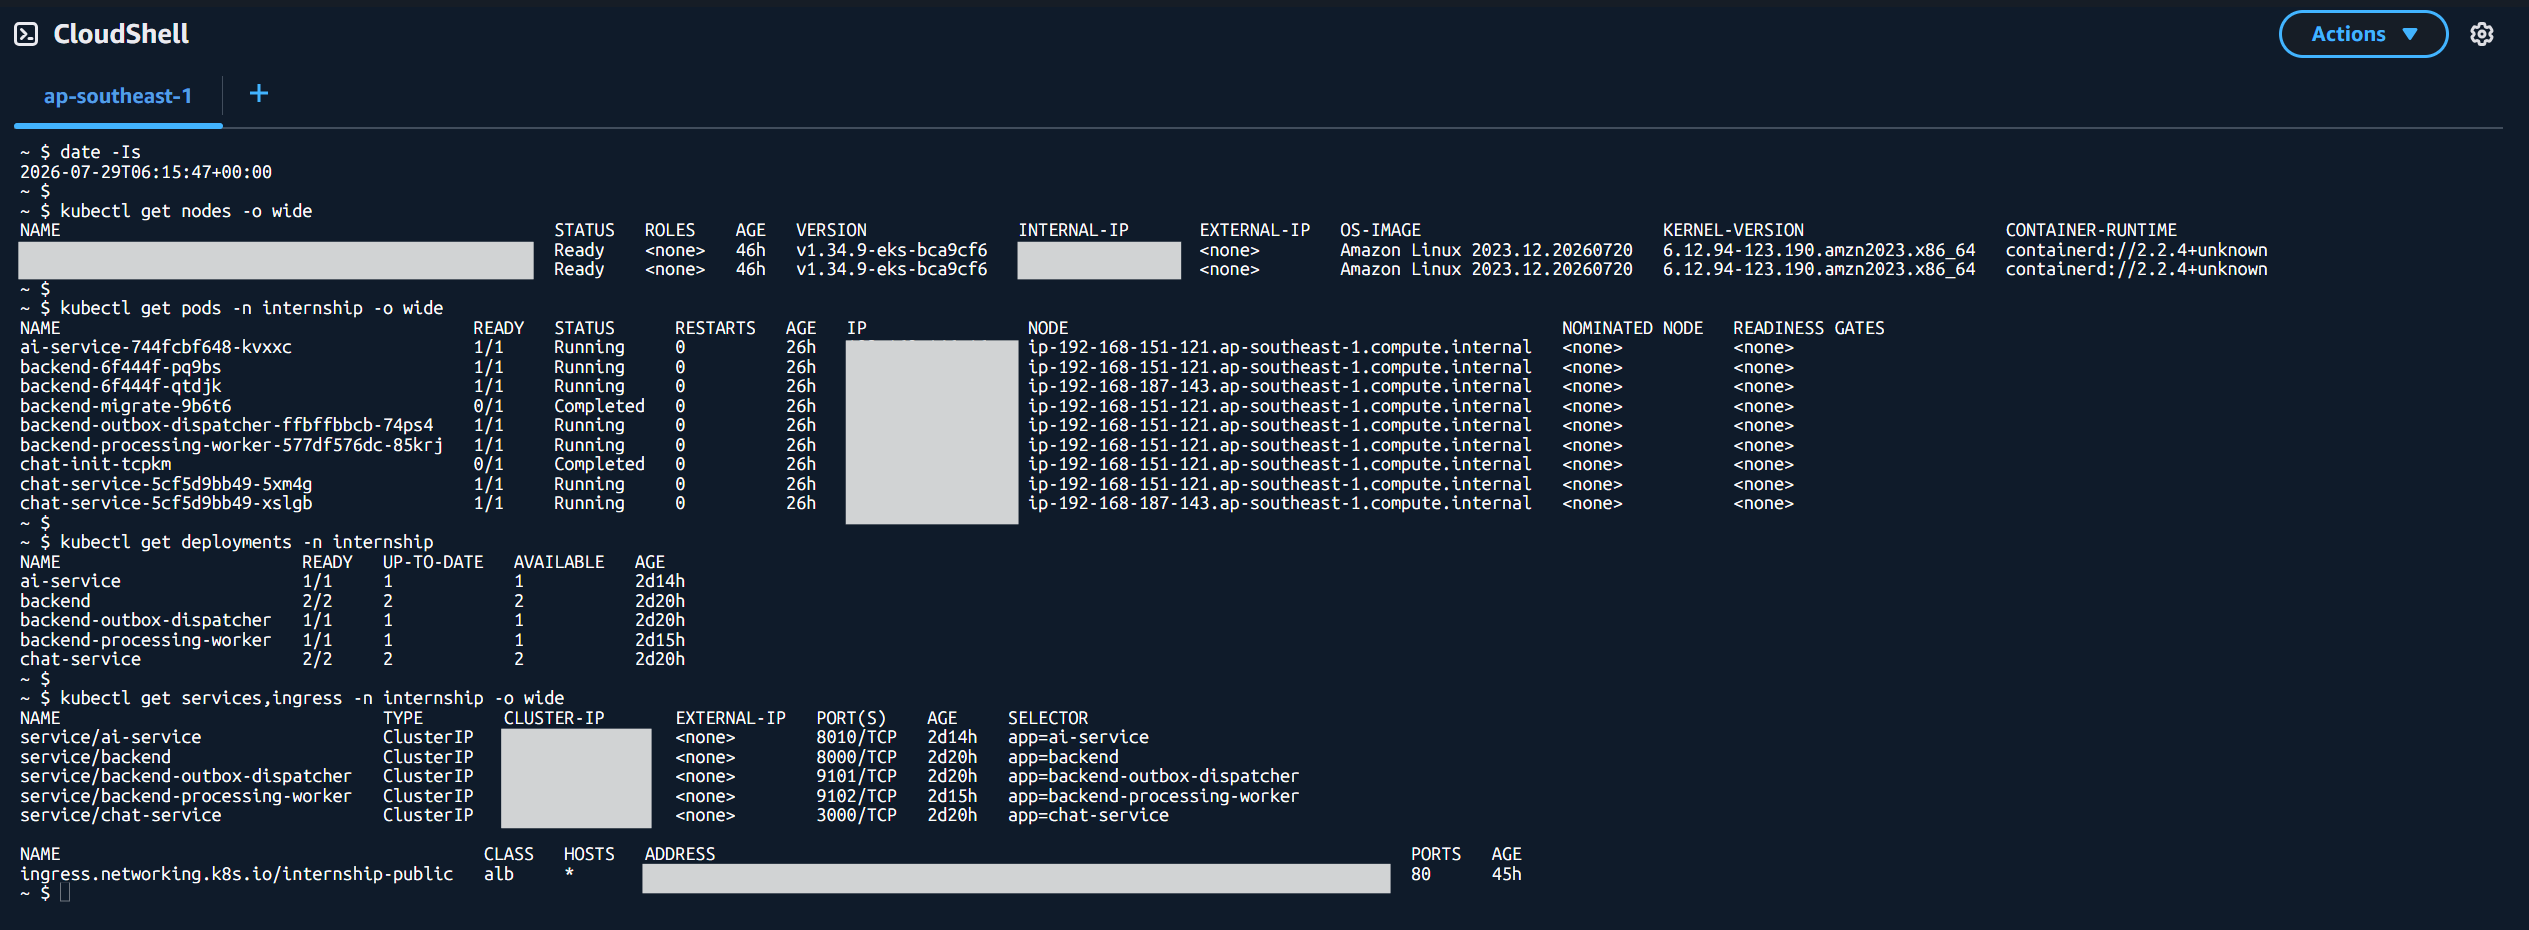
\includegraphics[keepaspectratio,alt={Amazon EKS runtime pods and services}]{../static/logs/worklog/week-08/aws/eks-runtime-pods-2026-07-28.png}}
\caption{Amazon EKS runtime pods and services}
\end{figure}

\begin{figure}
\centering
\pandocbounded{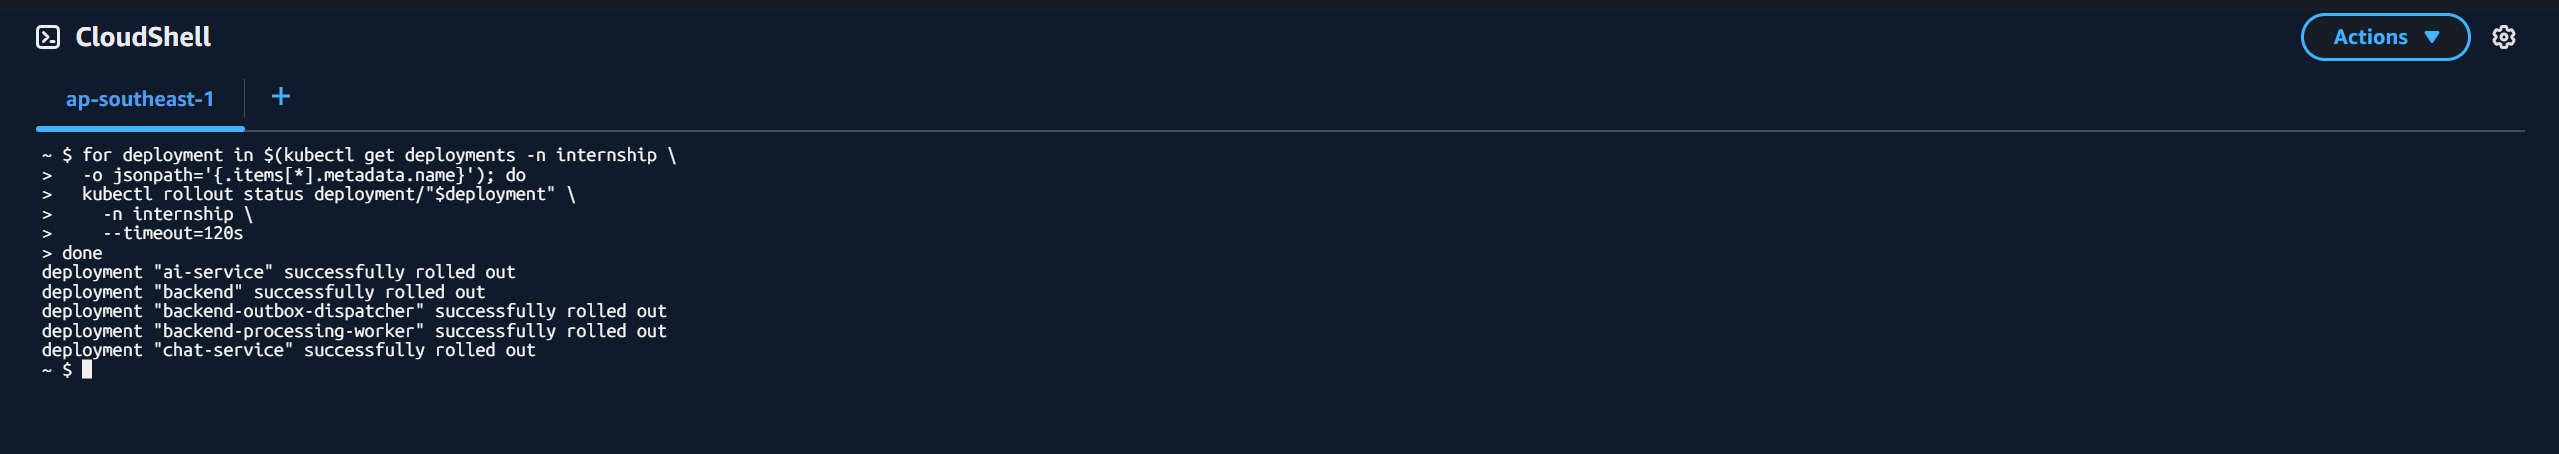
\includegraphics[keepaspectratio,alt={Amazon EKS deployment rollout success}]{../static/logs/worklog/week-08/aws/eks-deployment-rollout-success.png}}
\caption{Amazon EKS deployment rollout success}
\end{figure}

\vspace{0.5em}\noindent\textbf{Application Load
Balancer}\par

\textbf{Evidence status:} Available \textbf{Runtime status:} Partially
operational

I captured an internet-facing Application Load Balancer in
\texttt{active} state. However, the target health evidence still shows
mixed target status:

\begin{itemize}
\tightlist
\item
  One backend target on port \texttt{8000} was healthy.
\item
  Another backend target on port \texttt{8000} was unhealthy with failed
  health checks.
\item
  Chat targets on port \texttt{3000} were unhealthy with timeout or
  failed health-check reasons.
\end{itemize}

Because of the unhealthy targets, I do not classify the ALB as fully
healthy. The load balancer was deployed, active, and associated with
target groups, but the target groups still require follow-up validation
and remediation.

\begin{figure}
\centering
\pandocbounded{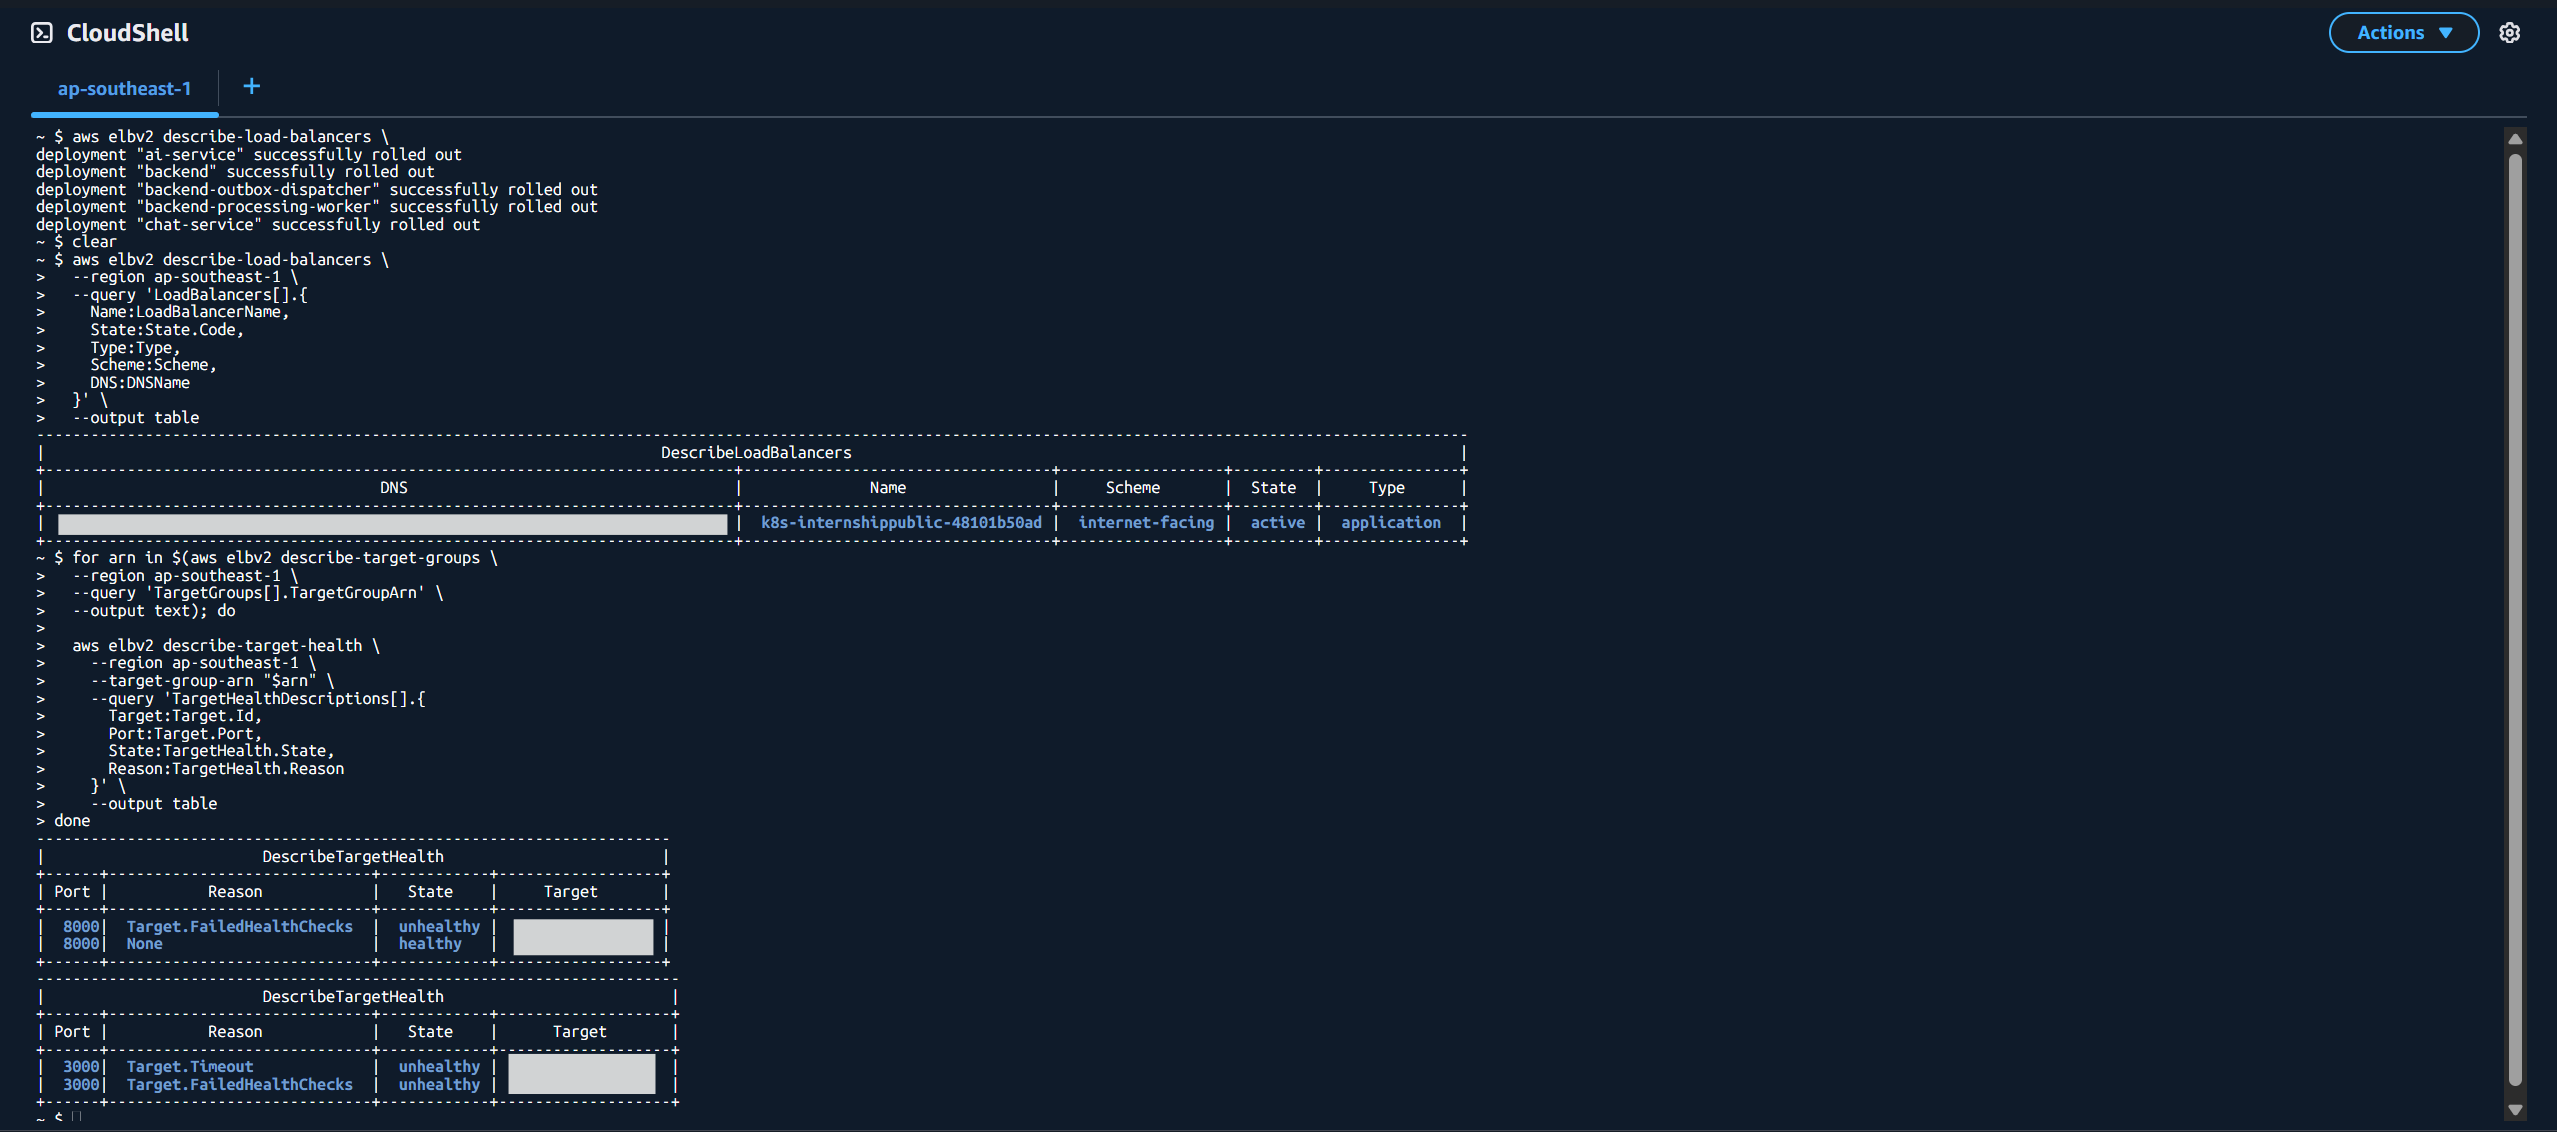
\includegraphics[keepaspectratio,alt={Application Load Balancer target health}]{../static/logs/worklog/week-08/aws/ALB-target-health.png}}
\caption{Application Load Balancer target health}
\end{figure}

\begin{figure}
\centering
\pandocbounded{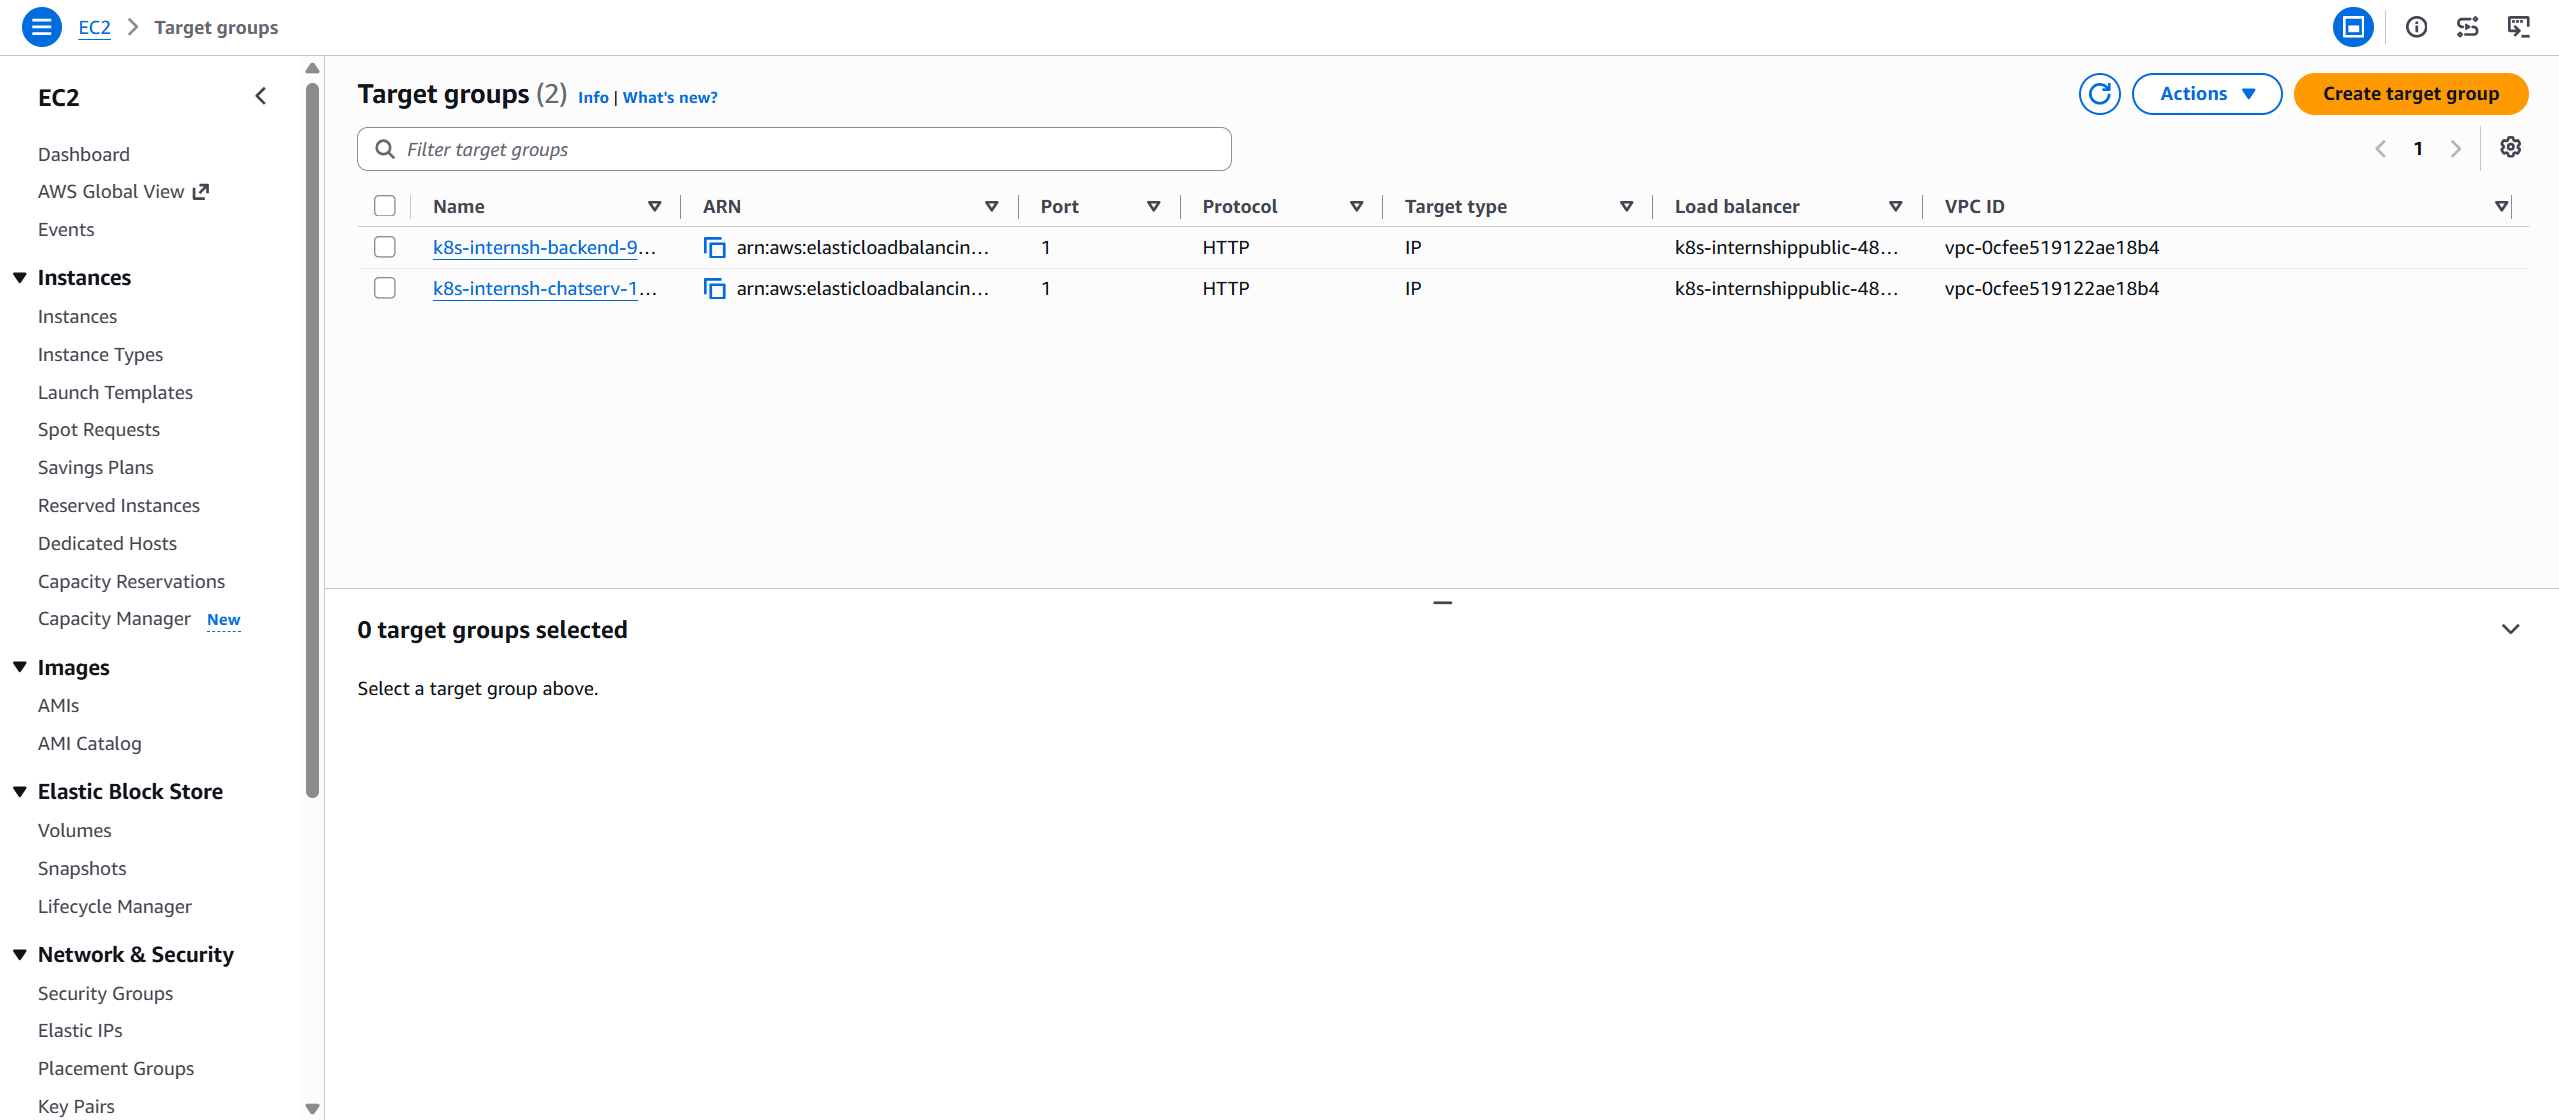
\includegraphics[keepaspectratio,alt={Application Load Balancer target groups}]{../static/logs/worklog/week-08/aws/ALB-target.png}}
\caption{Application Load Balancer target groups}
\end{figure}

\vspace{0.5em}\noindent\textbf{Amazon CloudFront and S3}\par

\textbf{Evidence status:} Available \textbf{Runtime status:} Partially
verified

I captured CloudFront monitoring metrics for distribution
\texttt{EQIGYNECXDYL8}, including requests, data transfer, and
error-rate graphs over the selected three-day window. This confirms that
the distribution was receiving telemetry.

I captured the frontend S3 bucket object listing after redacting the
bucket name. The visible objects include \texttt{assets/\allowbreak{}},
\texttt{favicon.\allowbreak{}svg}, and \texttt{index.\allowbreak{}html}, which verifies that
static frontend assets were present in S3.

These screenshots support frontend hosting evidence, but they do not
replace a full CloudFront behavior/origin configuration export or a
browser smoke test through the CloudFront URL.

\begin{figure}
\centering
\pandocbounded{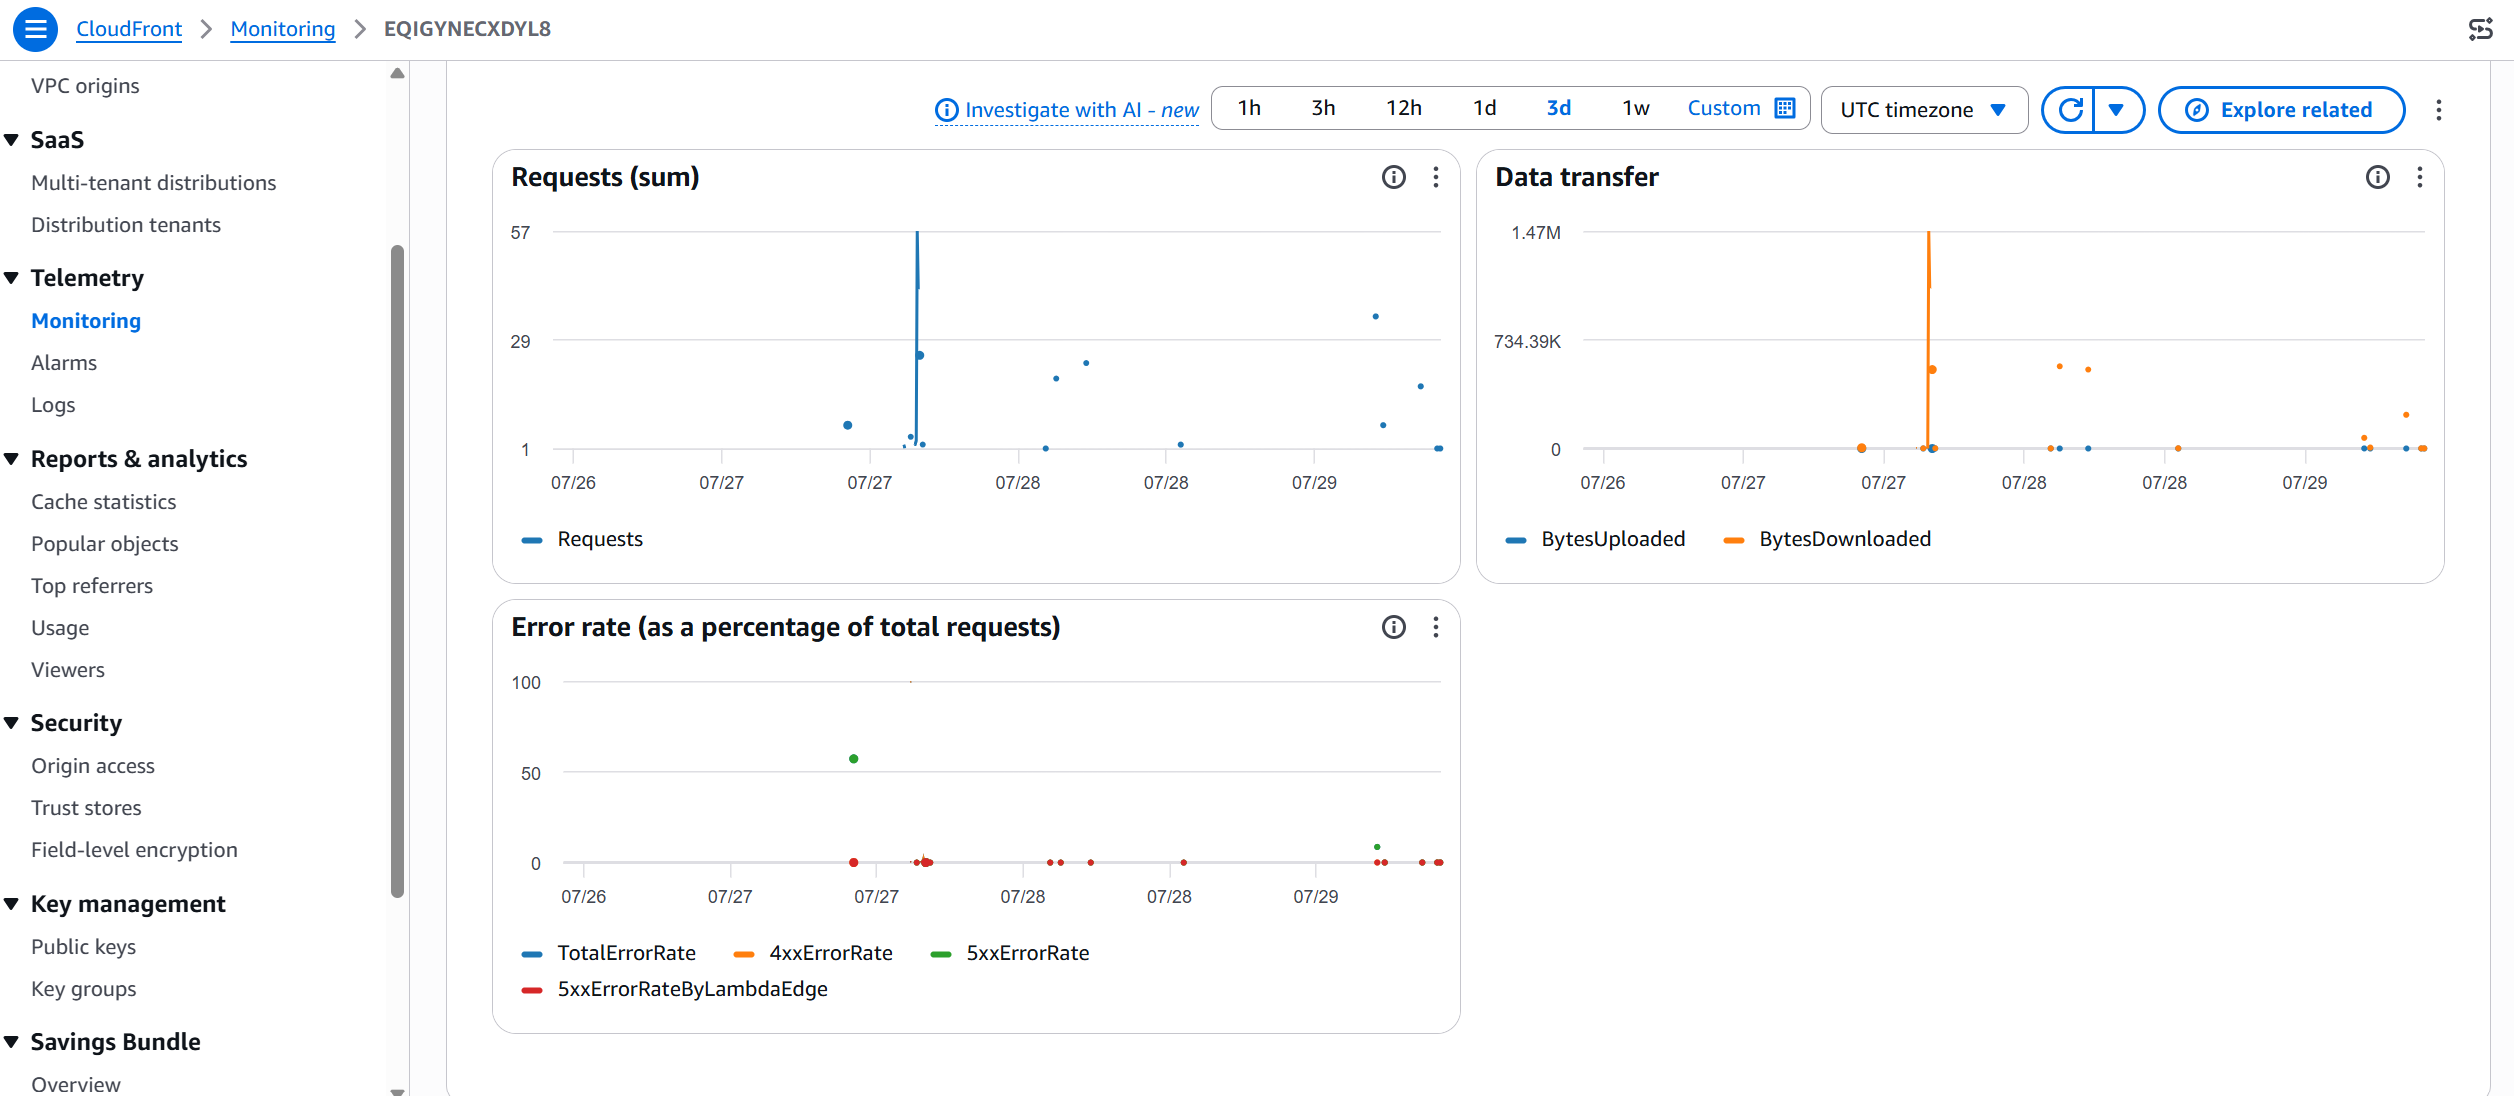
\includegraphics[keepaspectratio,alt={CloudFront monitoring evidence}]{../static/logs/worklog/week-08/aws/Cloudfront-evidence.png}}
\caption{CloudFront monitoring evidence}
\end{figure}

\begin{figure}
\centering
\pandocbounded{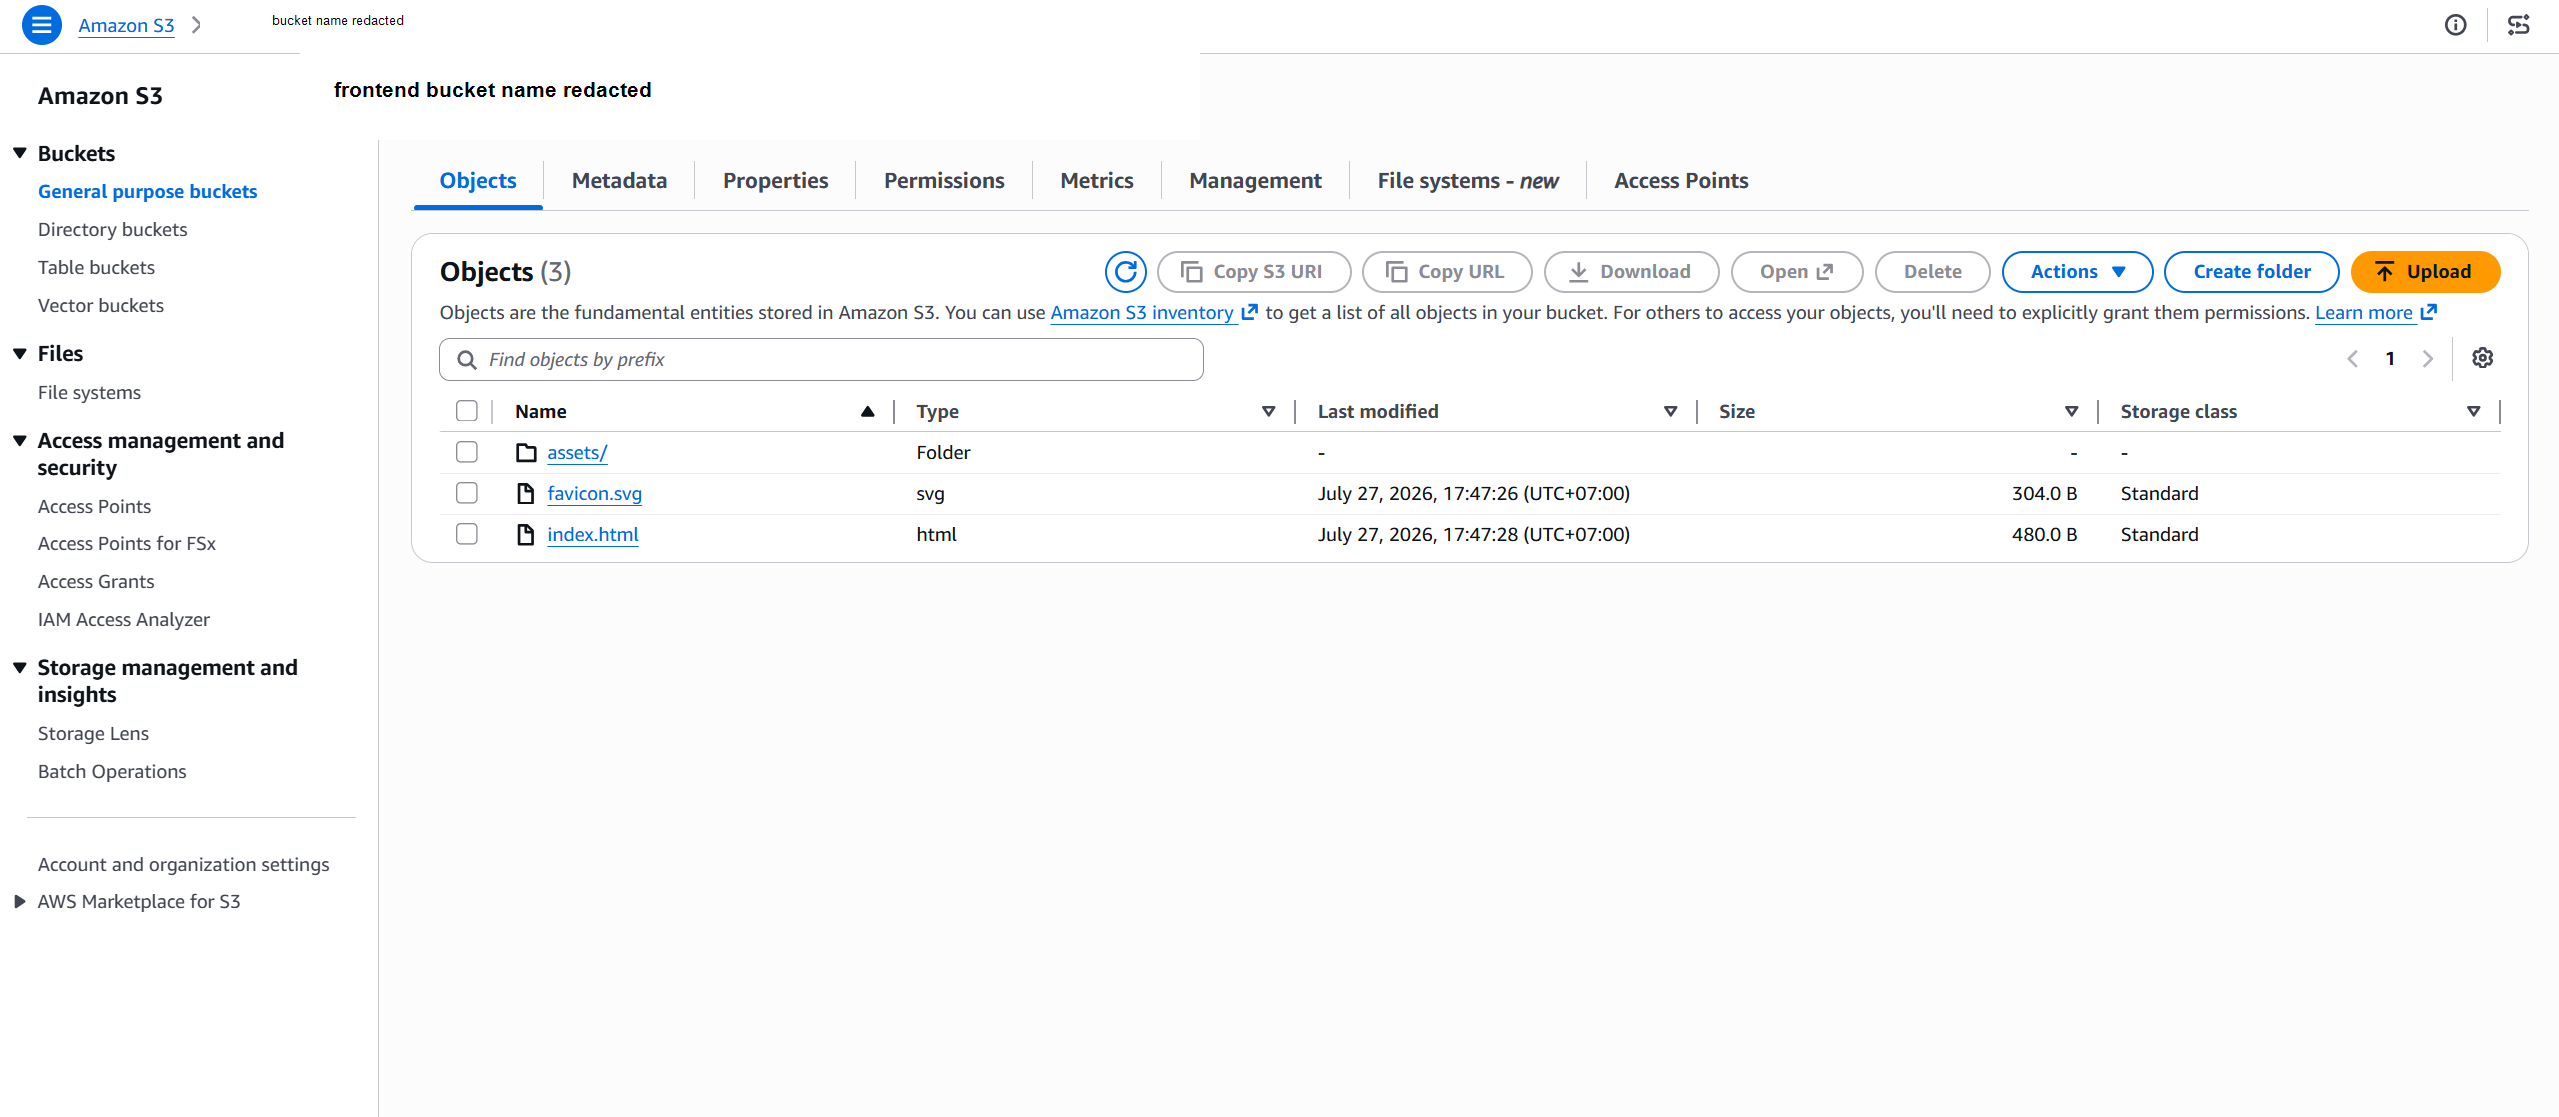
\includegraphics[keepaspectratio,alt={S3 frontend bucket object evidence}]{../static/logs/worklog/week-08/aws/S3-evidenc.png}}
\caption{S3 frontend bucket object evidence}
\end{figure}

\vspace{0.5em}\noindent\textbf{Amazon RDS}\par

\textbf{Evidence status:} Available \textbf{Runtime status:} Available

I verified the PostgreSQL database instance
\texttt{internship-\allowbreak{}prod-\allowbreak{}postgres} in status \texttt{available}. The
captured output also includes PostgreSQL engine metadata, encrypted
storage, non-public accessibility, and allocated storage.

\begin{figure}
\centering
\pandocbounded{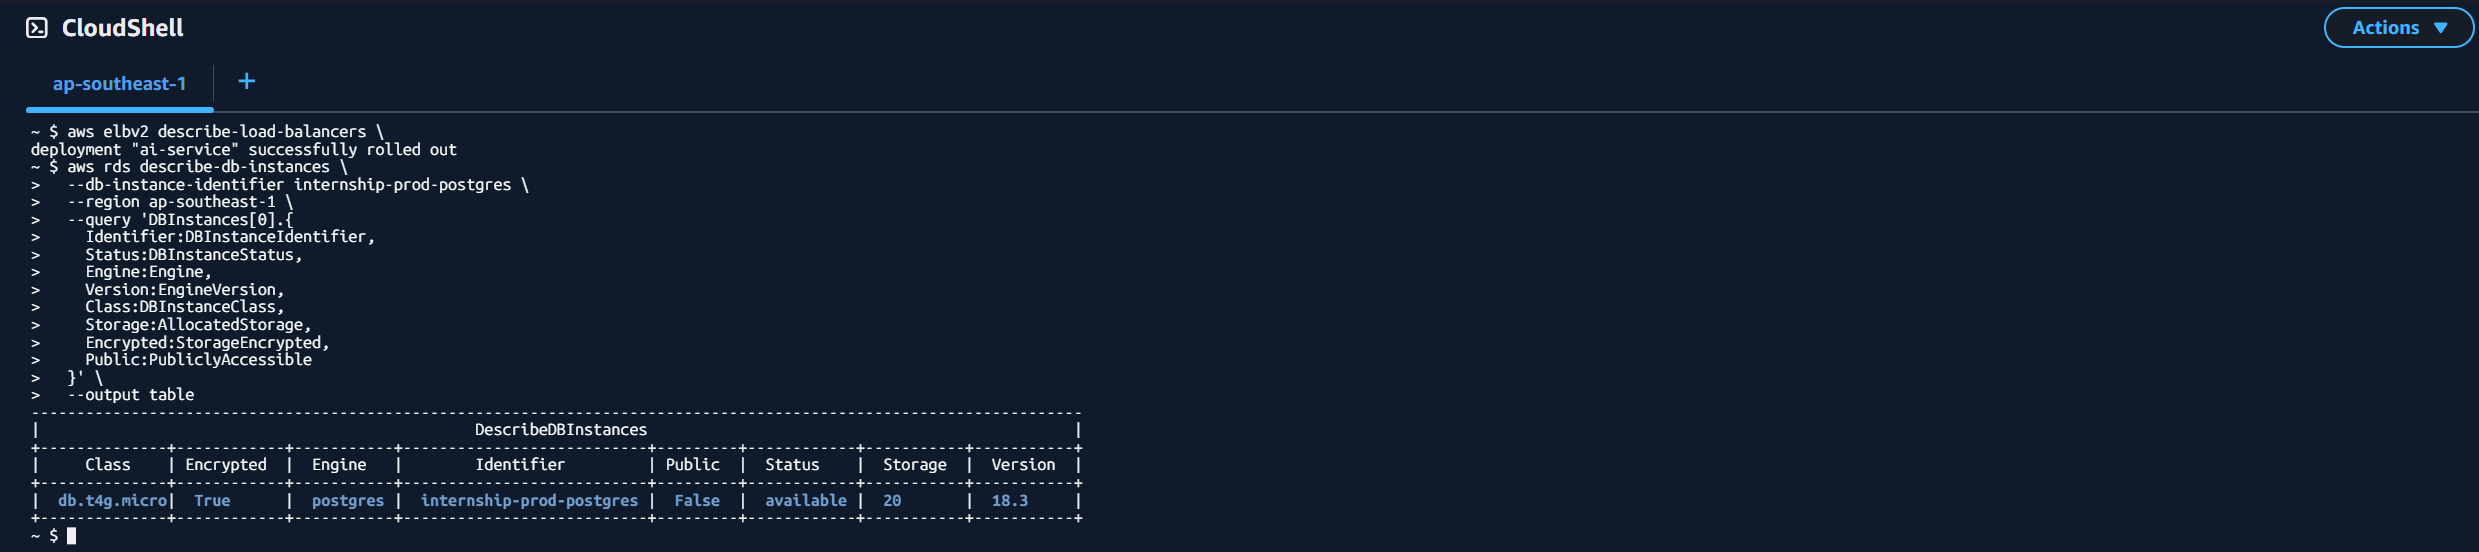
\includegraphics[keepaspectratio,alt={Amazon RDS PostgreSQL health}]{../static/logs/worklog/week-08/aws/RDS-health.png}}
\caption{Amazon RDS PostgreSQL health}
\end{figure}

\vspace{0.5em}\noindent\textbf{Amazon ElastiCache}\par

\textbf{Evidence status:} Available \textbf{Runtime status:} Available

I verified the ElastiCache replication group
\texttt{internship-\allowbreak{}prod-\allowbreak{}redis} with Valkey engine status
\texttt{available}. The captured evidence also confirms encryption at
rest and in transit.

\begin{figure}
\centering
\pandocbounded{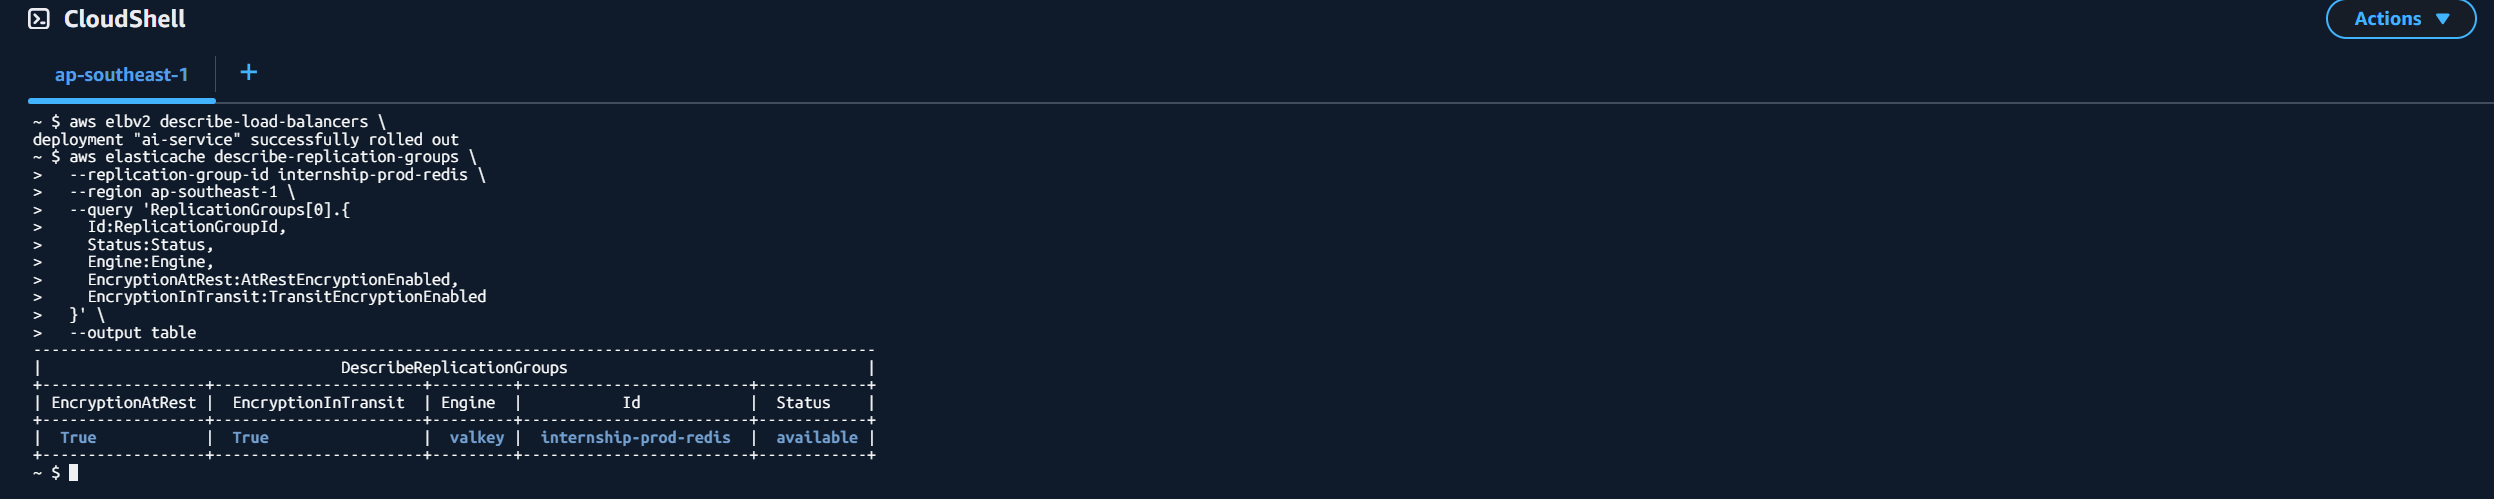
\includegraphics[keepaspectratio,alt={Amazon ElastiCache Valkey health}]{../static/logs/worklog/week-08/aws/REDIS-health.png}}
\caption{Amazon ElastiCache Valkey health}
\end{figure}

\vspace{0.5em}\noindent\textbf{Amazon DynamoDB}\par

\textbf{Evidence status:} Available \textbf{Runtime status:} Verified
Active

I verified four DynamoDB tables in \texttt{Active} status:

\begin{itemize}
\tightlist
\item
  \texttt{ChatGroups}
\item
  \texttt{ChatMessages}
\item
  \texttt{ChatUsers}
\item
  \texttt{InternshipLambdaEventDedupe}
\end{itemize}

The captured table list also shows on-demand read and write capacity
mode. This verifies that the AWS DynamoDB tables existed and were active
at the time of evidence collection.

\begin{figure}
\centering
\pandocbounded{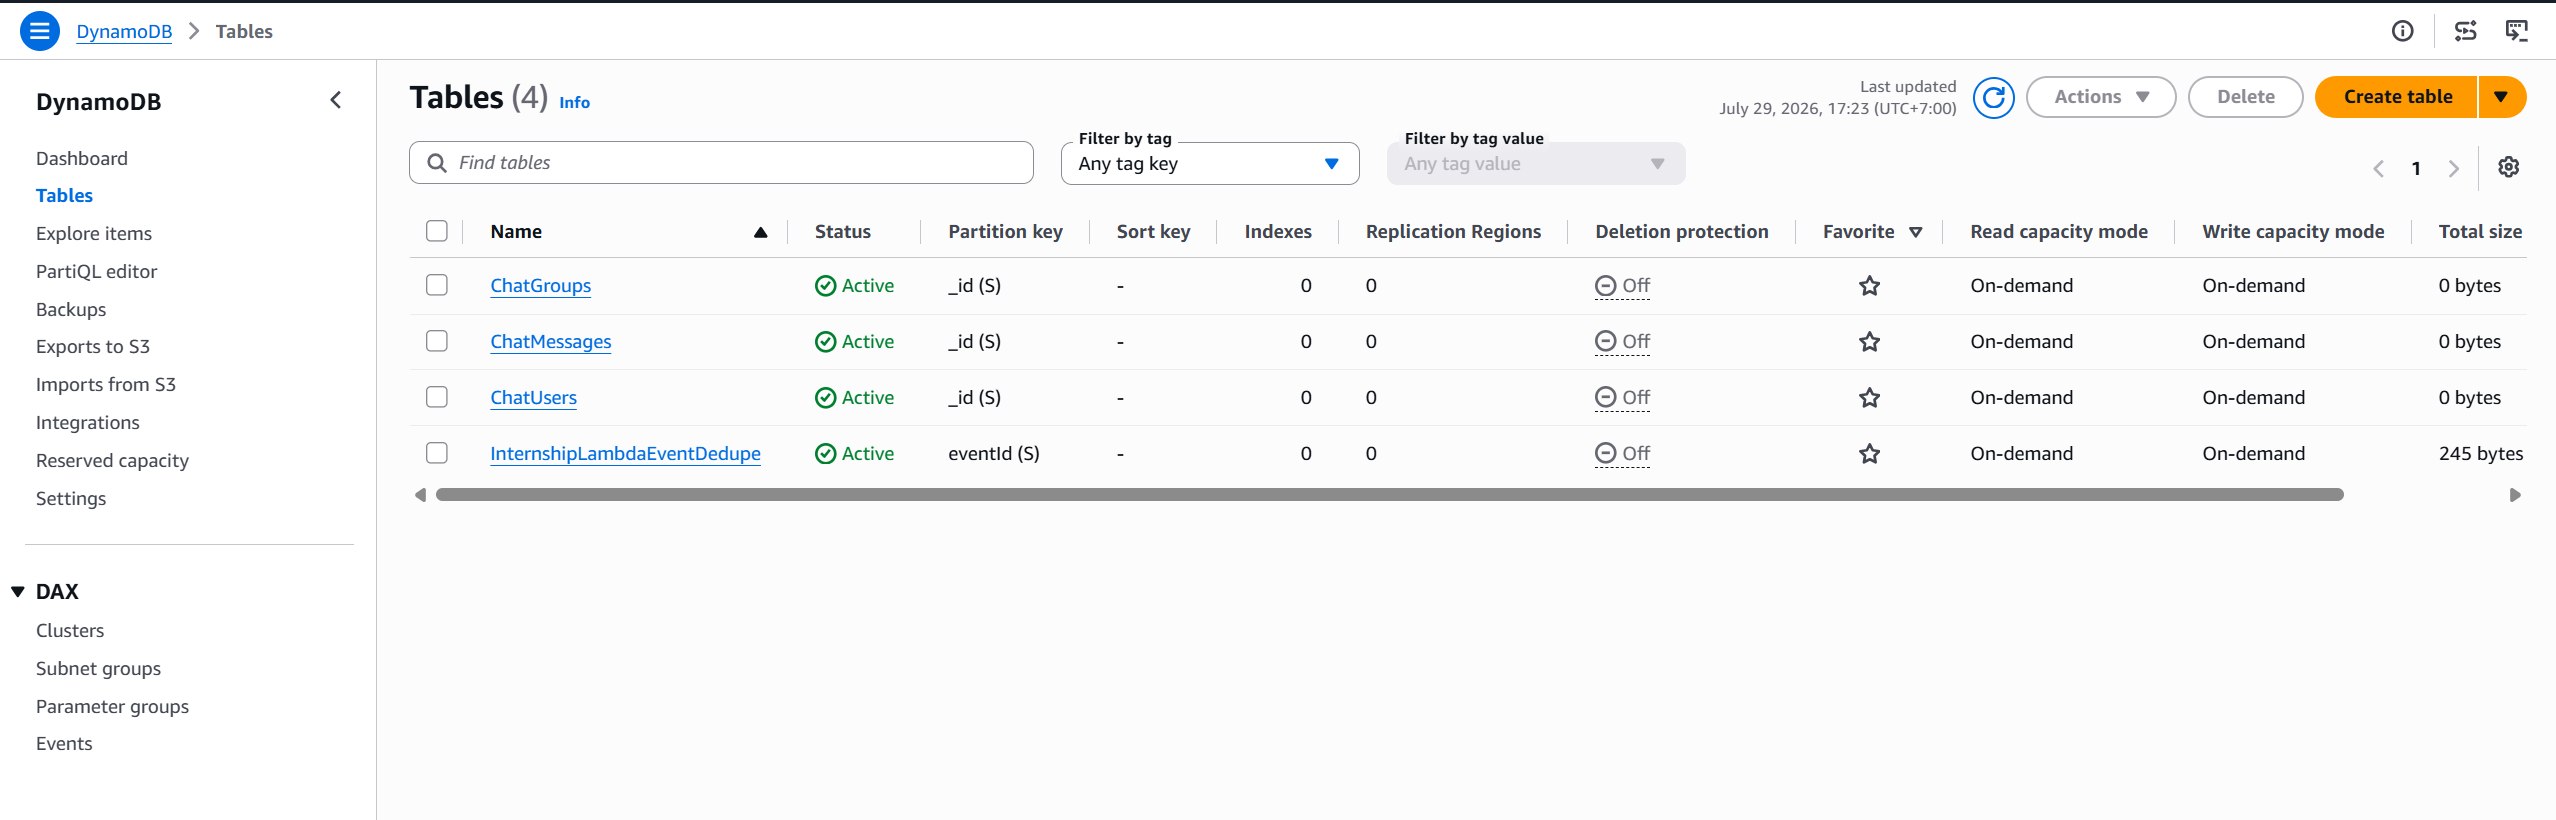
\includegraphics[keepaspectratio,alt={DynamoDB table status evidence}]{../static/logs/worklog/week-08/aws/DynamoDB-evidenc.png}}
\caption{DynamoDB table status evidence}
\end{figure}

\vspace{0.5em}\noindent\textbf{Amazon SQS}\par

\textbf{Evidence status:} Available \textbf{Runtime status:} Verified
available

I verified two Amazon SQS standard queues:

\begin{itemize}
\tightlist
\item
  \texttt{internship-\allowbreak{}prod-\allowbreak{}outbox}
\item
  \texttt{internship-\allowbreak{}prod-\allowbreak{}outbox-\allowbreak{}dlq}
\end{itemize}

Both queues had zero visible messages and zero in-flight messages in the
captured evidence. The queues use Amazon SQS managed server-side
encryption.

\begin{figure}
\centering
\pandocbounded{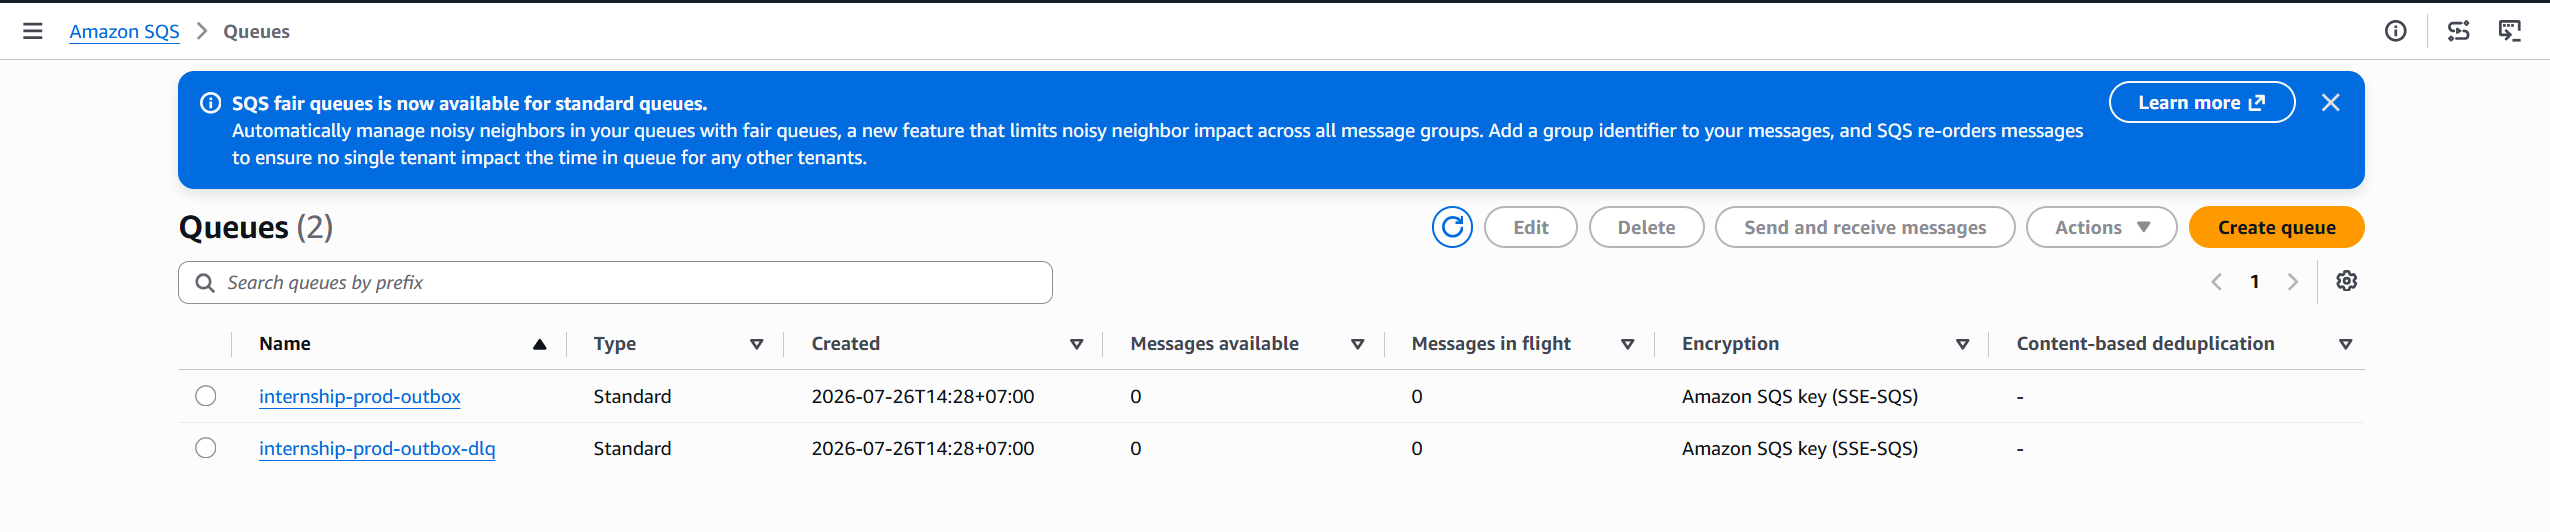
\includegraphics[keepaspectratio,alt={SQS queue evidence}]{../static/logs/worklog/week-08/aws/SQS-evidence.png}}
\caption{SQS queue evidence}
\end{figure}

\vspace{0.5em}\noindent\textbf{AWS Lambda}\par

\textbf{Evidence status:} Available \textbf{Runtime status:} Partially
verified

I verified a Lambda function named \texttt{internship-\allowbreak{}outbox-\allowbreak{}handler}
with a Python runtime and environment configuration. This confirms that
the function existed in the selected AWS region.

The screenshot was sanitized before publication by redacting
account-scoped ARNs, the IAM role ARN account segment, the bucket value
containing an account identifier, and the sender email address.

Additional Lambda evidence captures the function source view and a
CloudWatch log group named
\texttt{/\allowbreak{}aws/\allowbreak{}lambda/\allowbreak{}internship-\allowbreak{}outbox-\allowbreak{}handler}. These items confirm that
the function code view and log group existed. They do not prove a
successful invocation, SQS trigger execution, or SES delivery result, so
I keep Lambda runtime execution as partially verified.

\begin{figure}
\centering
\pandocbounded{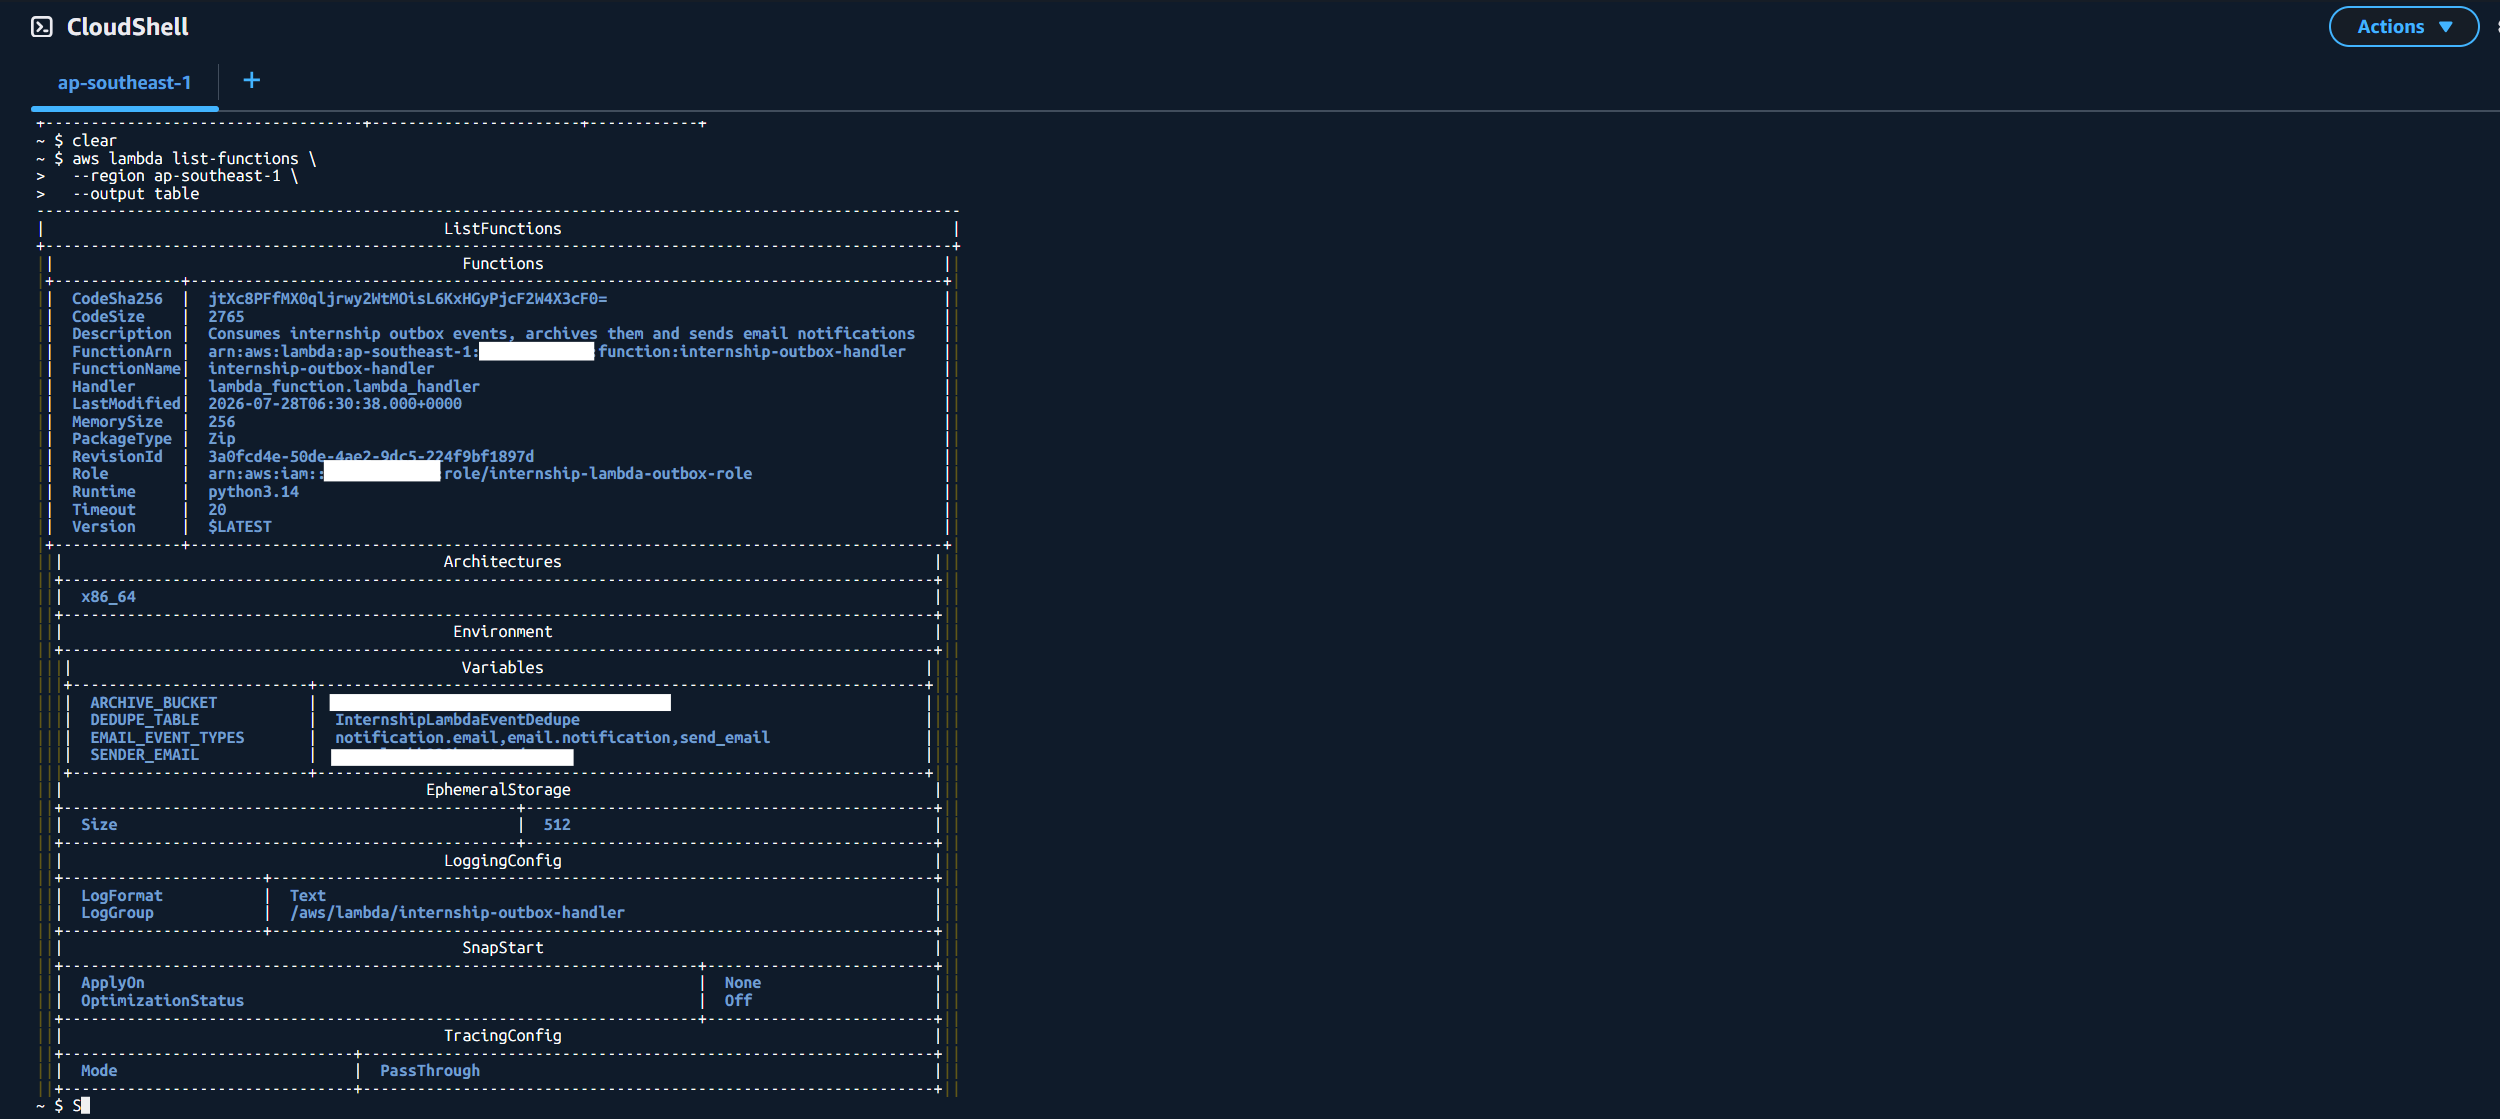
\includegraphics[keepaspectratio,alt={AWS Lambda function configuration}]{../static/logs/worklog/week-08/aws/lambda.png}}
\caption{AWS Lambda function configuration}
\end{figure}

\begin{figure}
\centering
\pandocbounded{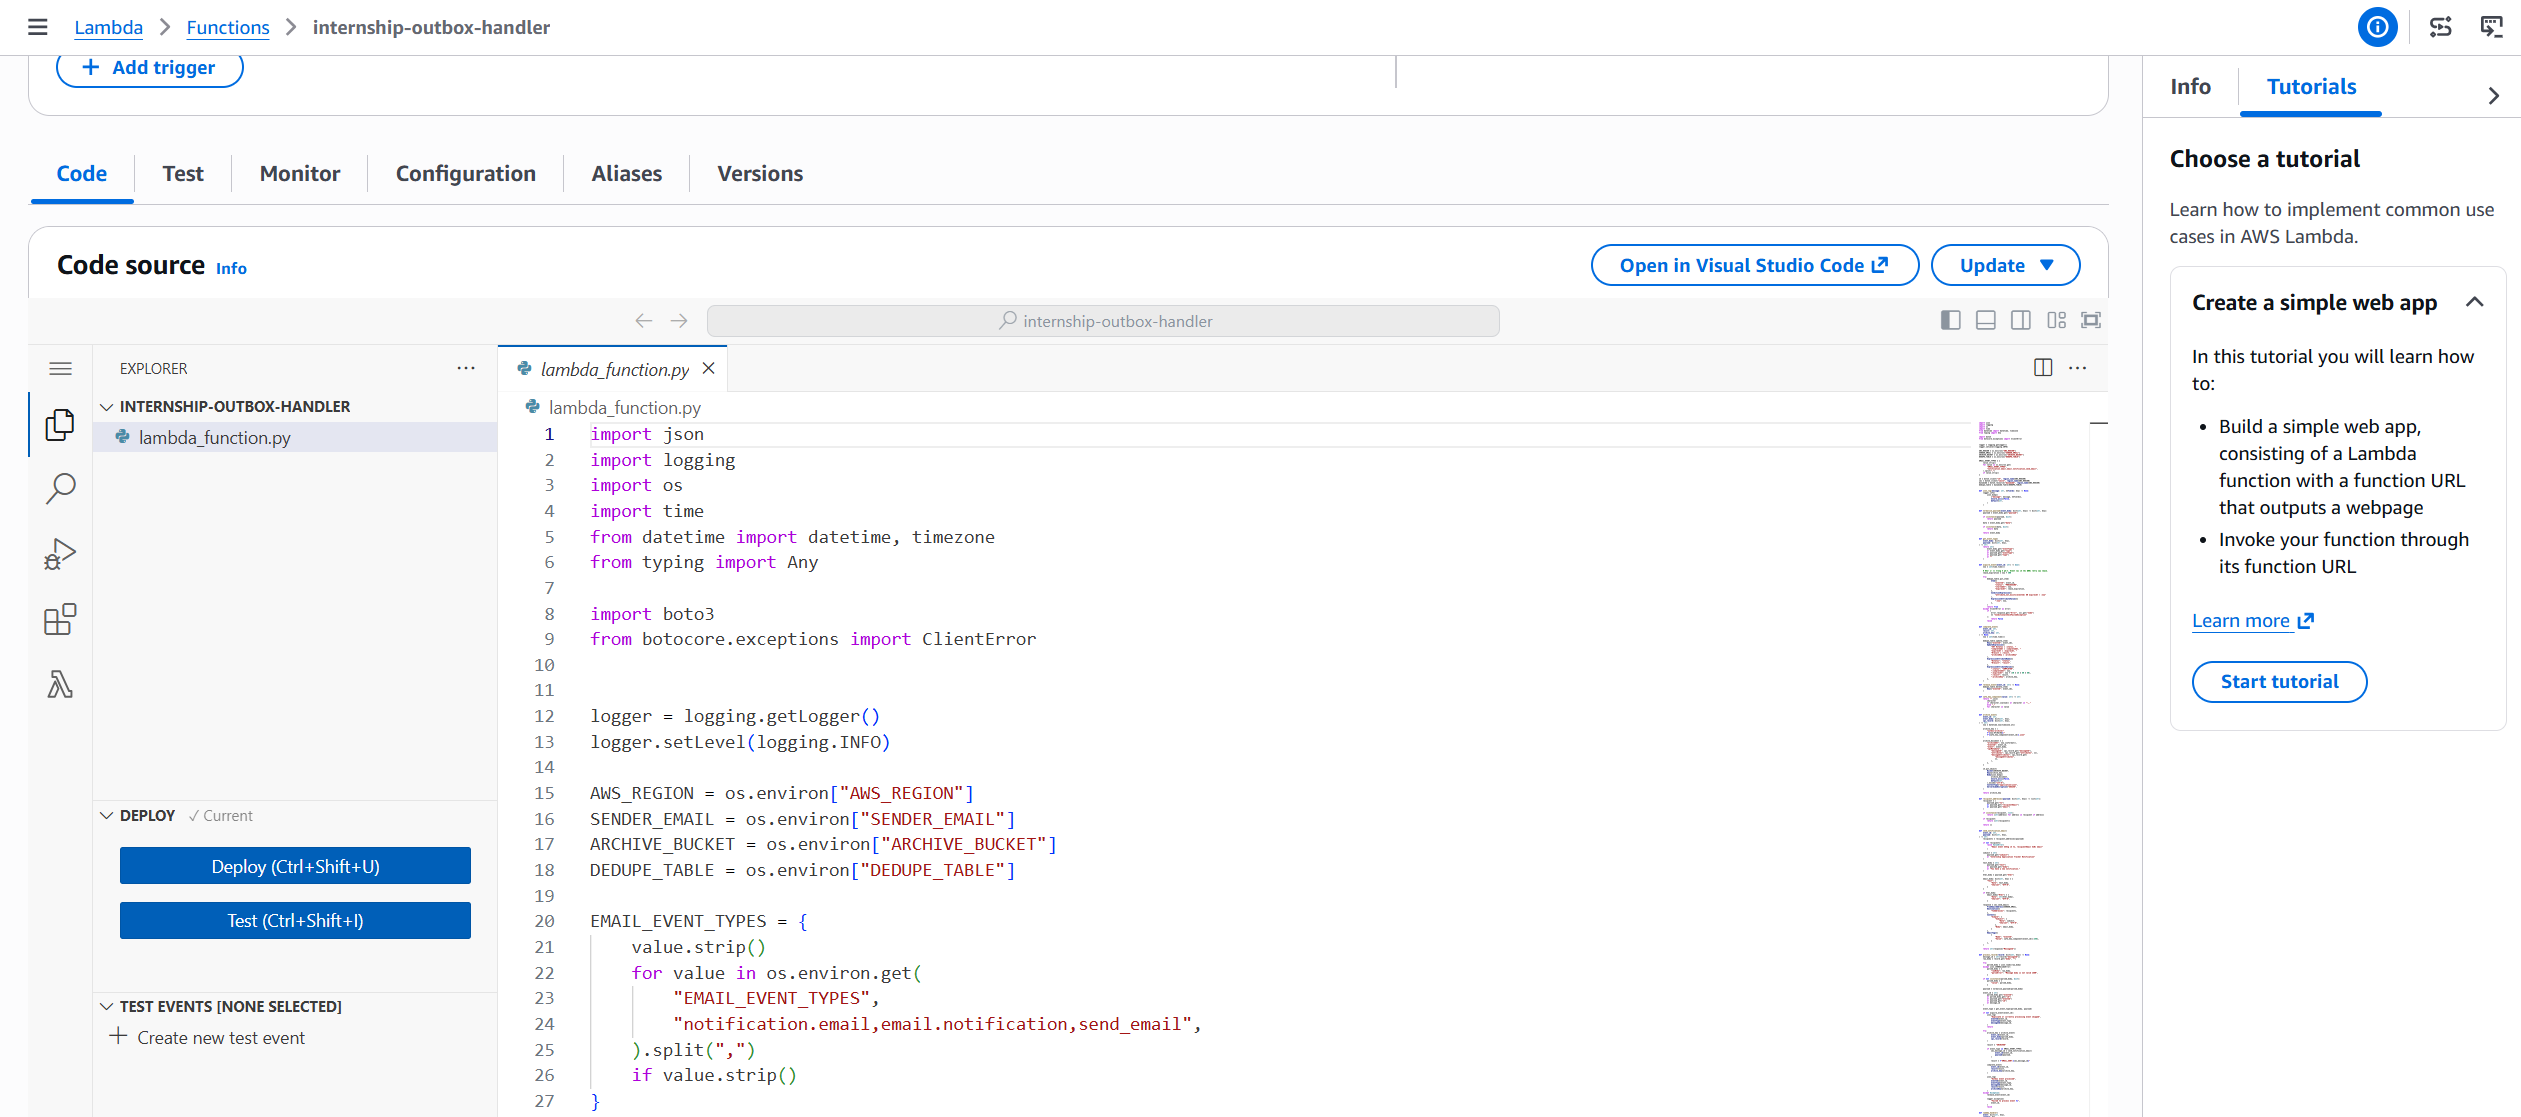
\includegraphics[keepaspectratio,alt={AWS Lambda source evidence}]{../static/logs/worklog/week-08/aws/Lambda-evidence.png}}
\caption{AWS Lambda source evidence}
\end{figure}

\begin{figure}
\centering
\pandocbounded{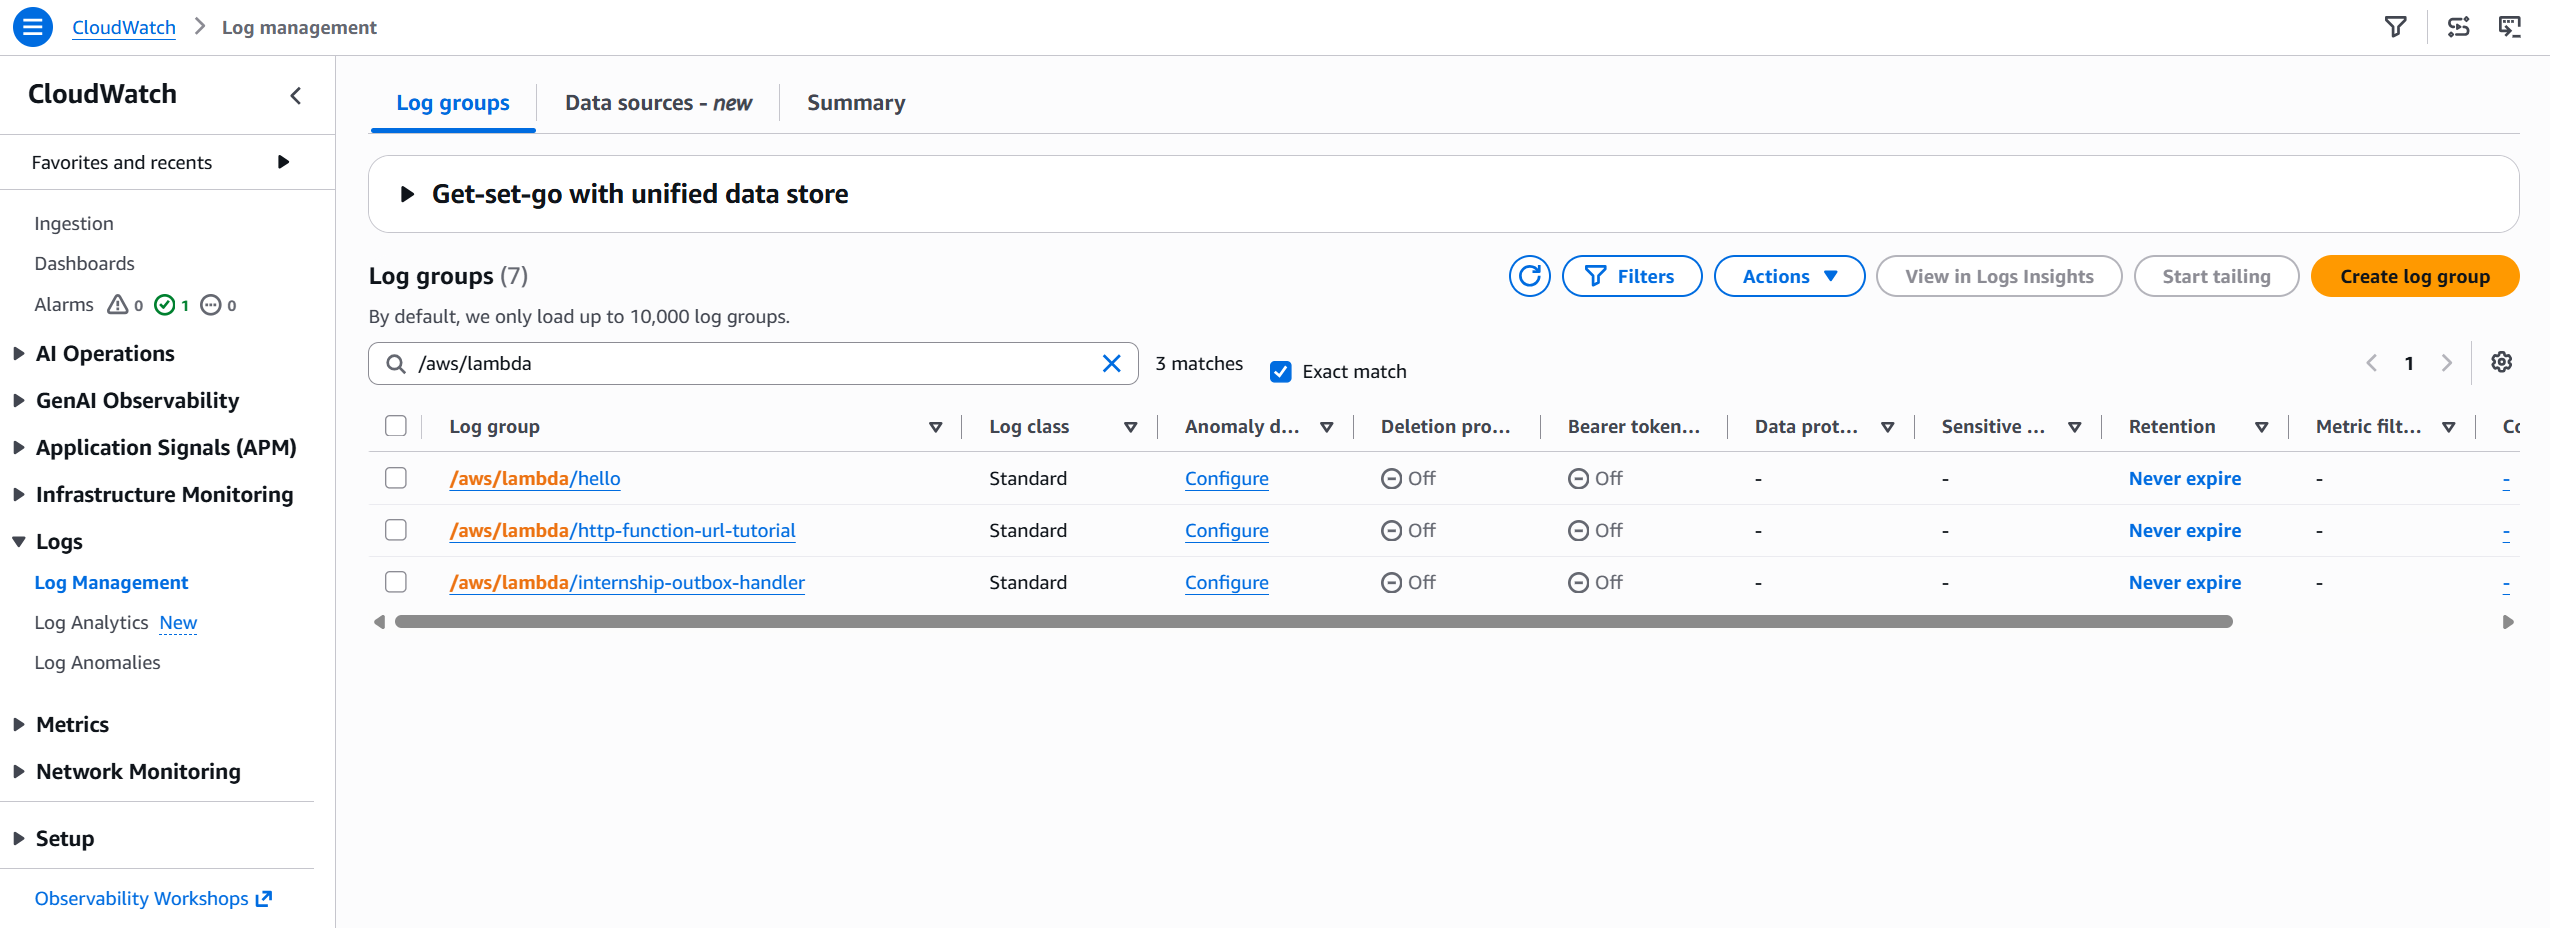
\includegraphics[keepaspectratio,alt={AWS Lambda CloudWatch log group evidence}]{../static/logs/worklog/week-08/aws/lambda-cloudwatch-evidence.png}}
\caption{AWS Lambda CloudWatch log group evidence}
\end{figure}

\vspace{0.5em}\noindent\textbf{Amazon SageMaker}\par

\textbf{Evidence status:} Available \textbf{Runtime status:} InService

I verified the SageMaker endpoint \texttt{internship-\allowbreak{}qwen3-\allowbreak{}4b} in status
\texttt{InService}. This is sufficient to show that the endpoint existed
and was serving at the time of evidence collection.

\begin{figure}
\centering
\pandocbounded{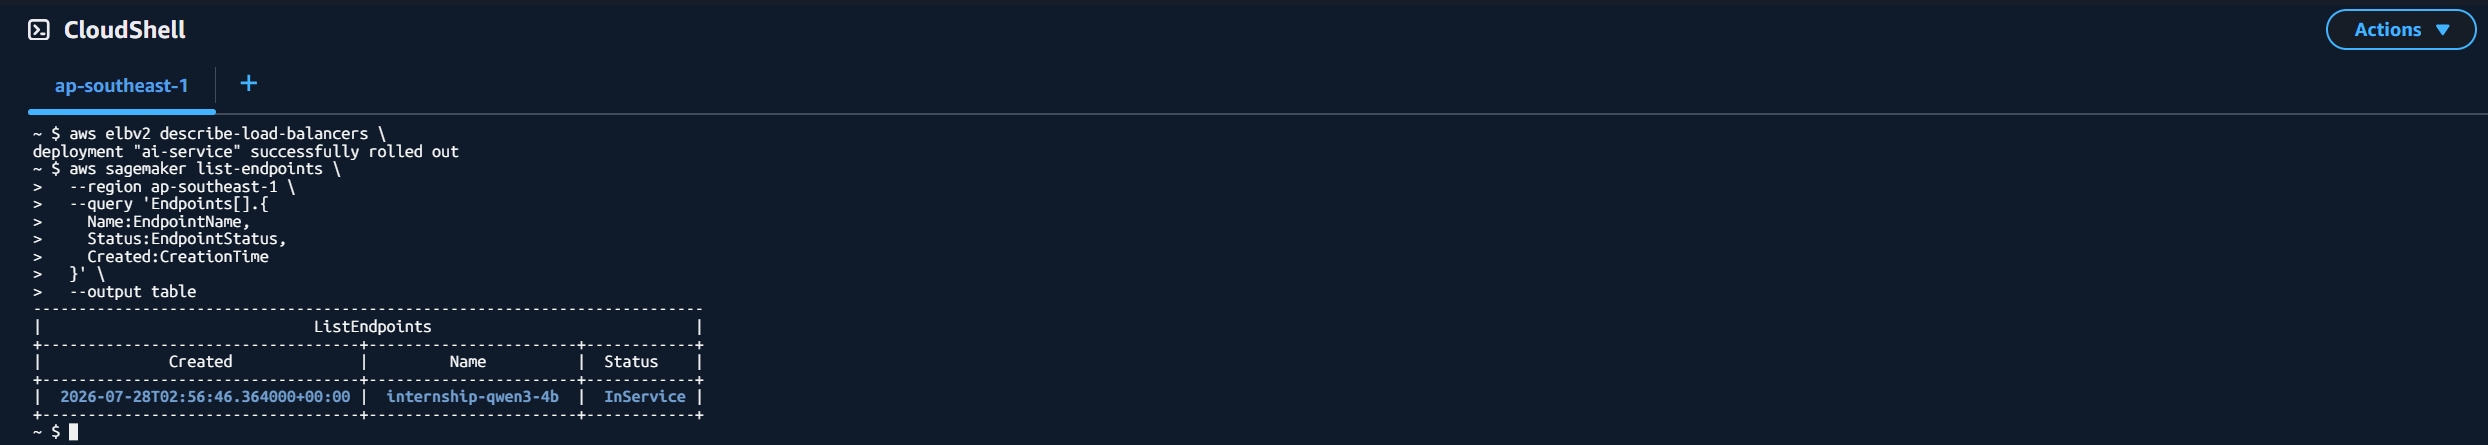
\includegraphics[keepaspectratio,alt={Amazon SageMaker endpoint status}]{../static/logs/worklog/week-08/aws/sagemaker-health.png}}
\caption{Amazon SageMaker endpoint status}
\end{figure}

\vspace{0.5em}\noindent\textbf{AWS Cost Evidence}\par

\begin{quote}
\textbf{Status: Partially available}
\end{quote}

The July 1-28, 2026 AWS cost summary reported a month-to-date spend of
\textbf{\$94.92}. I also included a Billing and Cost Management credits
screenshot stored as \texttt{total-\allowbreak{}cost-\allowbreak{}july.\allowbreak{}png} and a Cost Explorer
overview screenshot stored as \texttt{Cost-\allowbreak{}evidence.\allowbreak{}png}.

The credits screenshot records AWS credits rather than a grouped Cost
Explorer service chart. The Cost Explorer screenshot is useful as a
billing-console overview, but it uses a different report configuration
and is not a Pricing Calculator estimate. Therefore, I keep the
service-level cost breakdown tied to the July 1-28 cost summary.

\begin{figure}
\centering
\pandocbounded{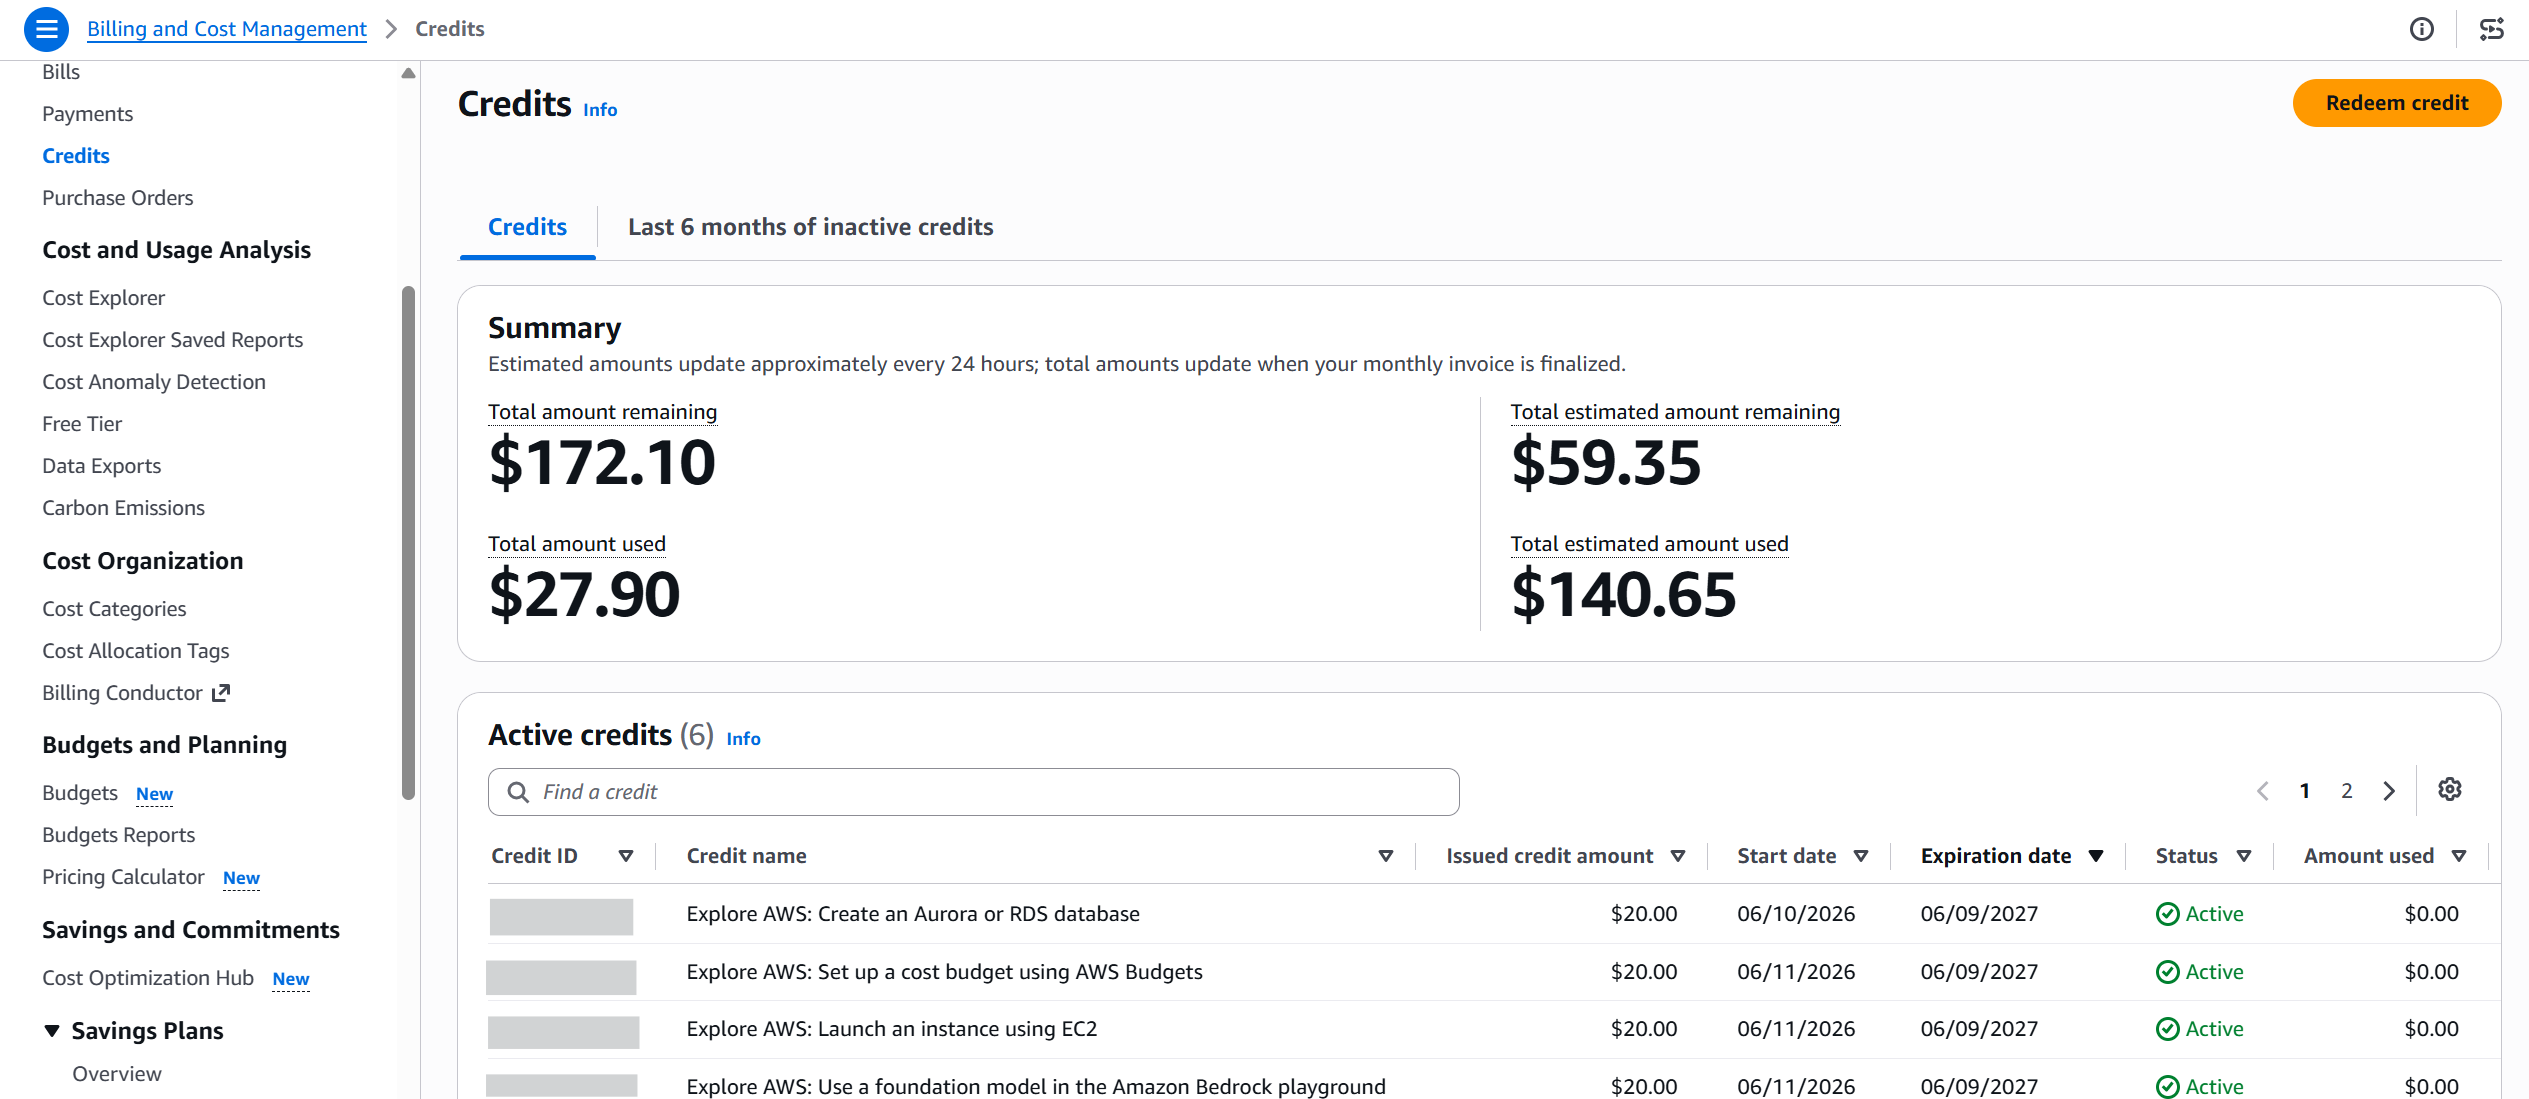
\includegraphics[keepaspectratio,alt={AWS Billing credits summary for July 2026}]{../static/logs/worklog/week-08/aws/total-cost-july.png}}
\caption{AWS Billing credits summary for July 2026}
\end{figure}

\begin{figure}
\centering
\pandocbounded{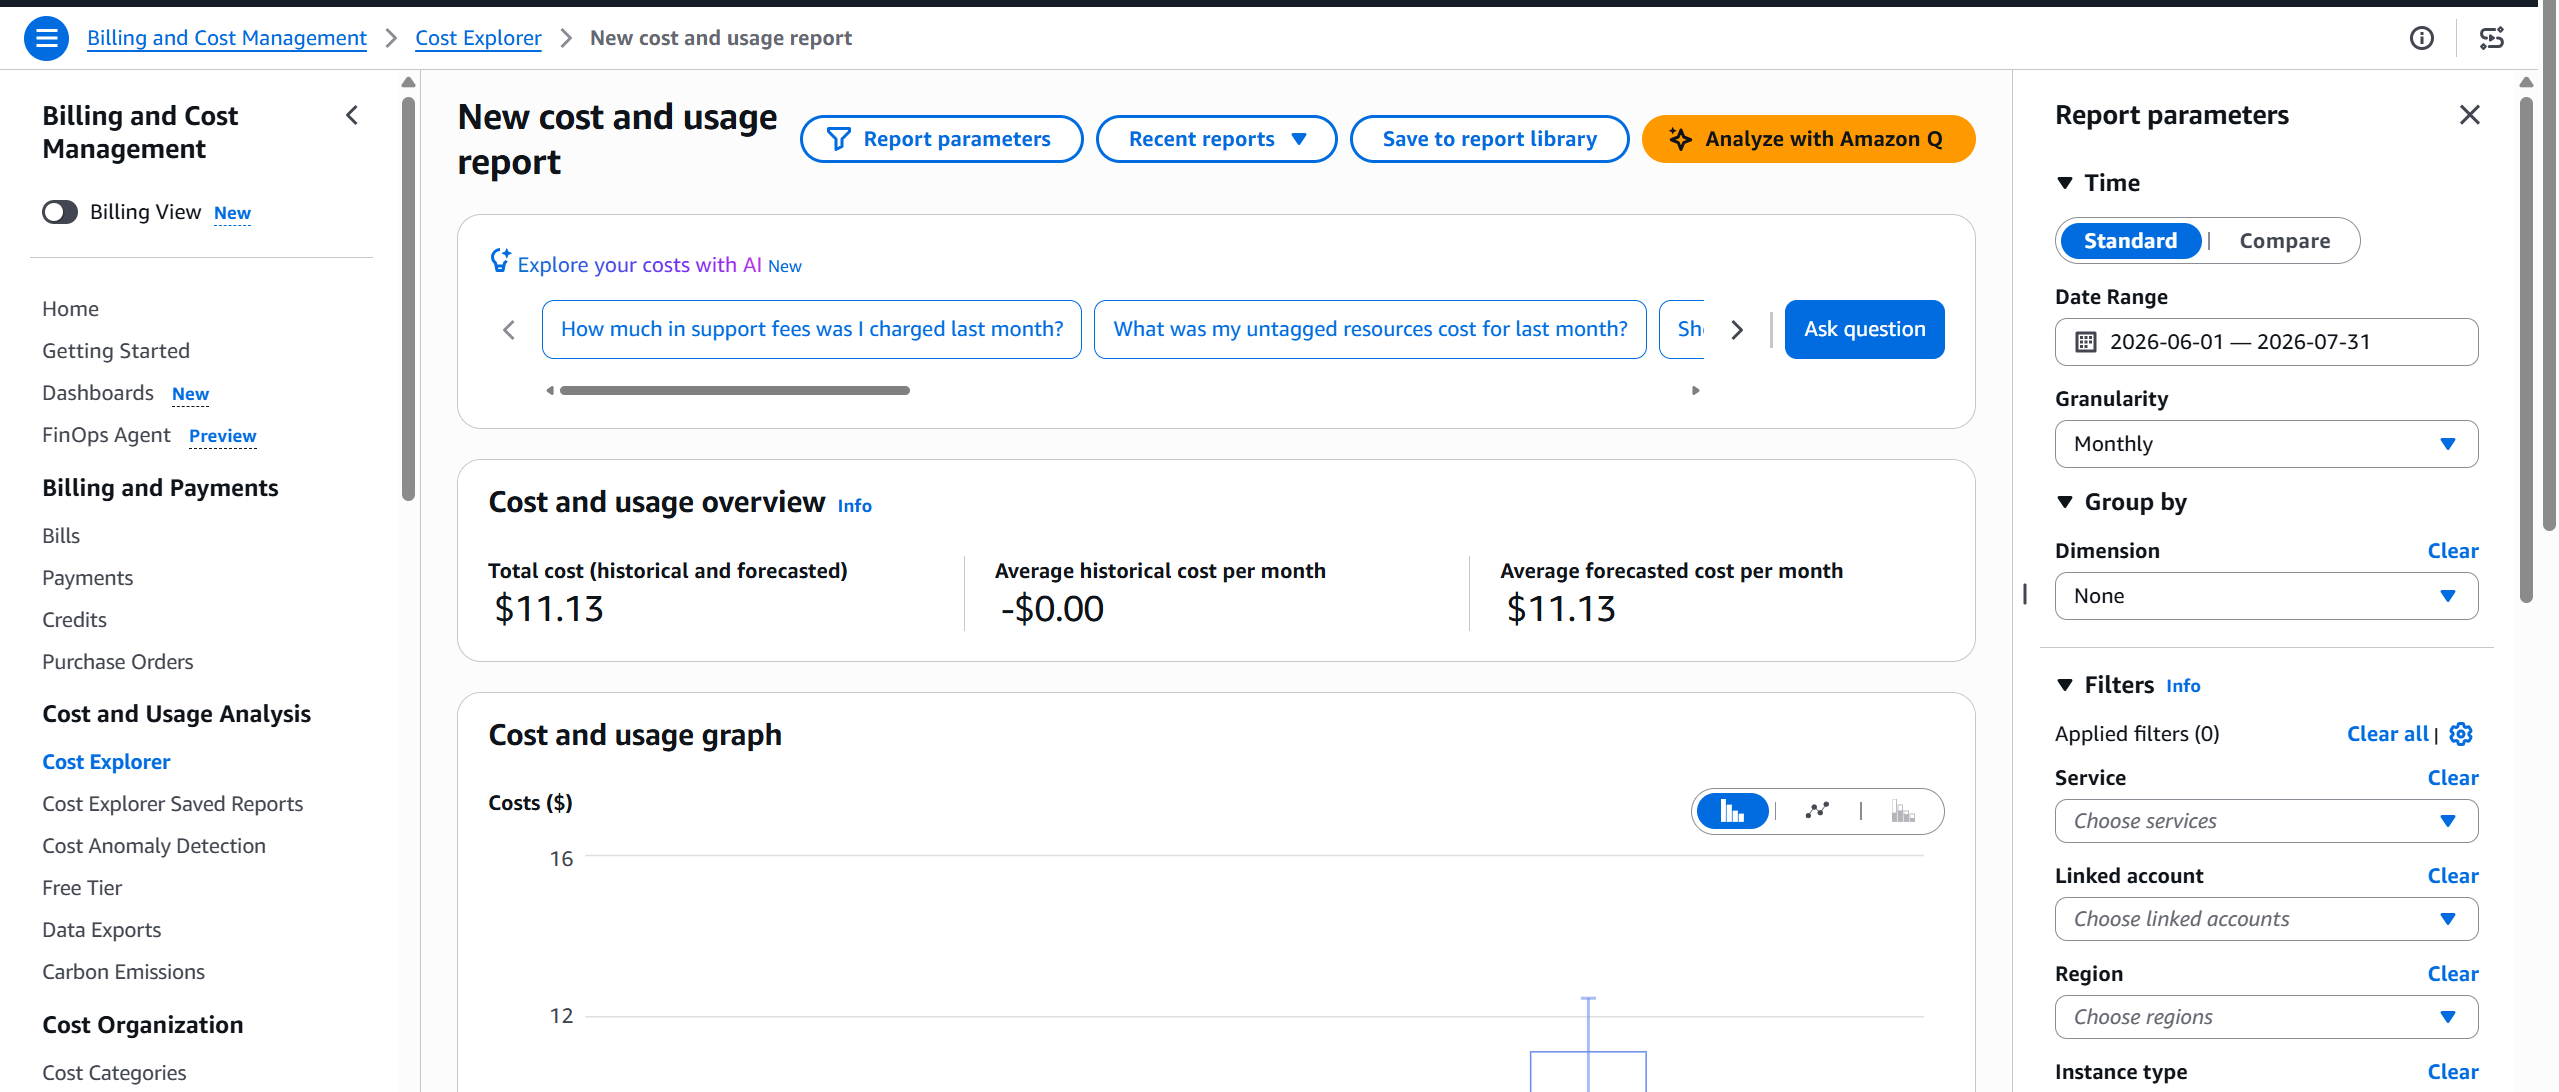
\includegraphics[keepaspectratio,alt={AWS Cost Explorer overview evidence}]{../static/logs/worklog/week-08/aws/Cost-evidence.png}}
\caption{AWS Cost Explorer overview evidence}
\end{figure}

\vspace{0.5em}\noindent\textbf{July 1-28 cost summary}\par

{
\begingroup
\small
\setlength{\tabcolsep}{3pt}
\renewcommand{\arraystretch}{1.15}
\begin{longtable}{@{}lr@{}}
\toprule\noalign{}
Metric & Reported value \\
\midrule\noalign{}
\endhead
\bottomrule\noalign{}
\endlastfoot
Total spend, July 1-28 & \$94.92 \\
Highest daily spend & \$31.83 on July 28 \\
AWS credits total amount used & \$27.90 \\
AWS credits total estimated amount used & \$140.65 \\
AWS credits total amount remaining & \$172.10 \\
AWS credits total estimated amount remaining & \$59.35 \\
\end{longtable}
\endgroup
}

\vspace{0.5em}\noindent\textbf{Daily cost trend}\par

{
\begingroup
\small
\setlength{\tabcolsep}{3pt}
\renewcommand{\arraystretch}{1.15}
\begin{longtable}{@{}lr@{}}
\toprule\noalign{}
Period & Daily spend \\
\midrule\noalign{}
\endhead
\bottomrule\noalign{}
\endlastfoot
July 1-8 & Approximately \$2.20/day \\
July 9-25 & Approximately \$1.60/day \\
July 26 & \$5.61 \\
July 27 & \$11.60 \\
July 28 & \$31.83 \\
\end{longtable}
\endgroup
}

The July 28 daily cost was the largest reported daily spend in the July
1-28 period and was much higher than the earlier baseline.

\vspace{0.5em}\noindent\textbf{Top cost drivers}\par

{
\begingroup
\small
\setlength{\tabcolsep}{3pt}
\renewcommand{\arraystretch}{1.15}
\begin{longtable}{@{}rlrr@{}}
\toprule\noalign{}
Rank & Service & Month-to-date cost & Share of total \\
\midrule\noalign{}
\endhead
\bottomrule\noalign{}
\endlastfoot
1 & Amazon RDS & \$29.69 & 31.3\% \\
2 & Amazon SageMaker & \$23.45 & 24.7\% \\
3 & Amazon VPC & \$14.11 & 14.9\% \\
4 & Amazon EC2 - Compute & \$12.42 & 13.1\% \\
5 & EC2 - Other & \$7.68 & 8.1\% \\
6 & Amazon EKS & \$5.64 & 5.9\% \\
\end{longtable}
\endgroup
}

These six services account for approximately 98\% of the July 1-28
reported spend.

\vspace{0.5em}\noindent\textbf{Cost anomalies}\par

Five active anomalies were reported around July 26-28 in
\texttt{ap-\allowbreak{}southeast-\allowbreak{}1}:

{
\begingroup
\small
\setlength{\tabcolsep}{3pt}
\renewcommand{\arraystretch}{1.15}
\begin{longtable}{@{}
  >{\raggedright\arraybackslash}p{(\linewidth - 4\tabcolsep) * \real{0.3000}}
  >{\raggedleft\arraybackslash}p{(\linewidth - 4\tabcolsep) * \real{0.4000}}
  >{\raggedright\arraybackslash}p{(\linewidth - 4\tabcolsep) * \real{0.3000}}@{}}
\toprule\noalign{}
\begin{minipage}[b]{\linewidth}\raggedright
Service
\end{minipage} & \begin{minipage}[b]{\linewidth}\raggedleft
Anomaly impact
\end{minipage} & \begin{minipage}[b]{\linewidth}\raggedright
Reported context
\end{minipage} \\
\midrule\noalign{}
\endhead
\bottomrule\noalign{}
\endlastfoot
Amazon EBS & +\$6.02, +15,050\% versus expected & NAT Gateway activity
in \texttt{ap-\allowbreak{}southeast-\allowbreak{}1} \\
Amazon EC2 - Compute & +\$2.56, +400\% versus expected & New
\texttt{t3.\allowbreak{}medium} instances in \texttt{ap-\allowbreak{}southeast-\allowbreak{}1} \\
Amazon RDS & +\$1.12, +138\% versus expected & New \texttt{db.\allowbreak{}t4g.\allowbreak{}micro}
instance activity in \texttt{ap-\allowbreak{}southeast-\allowbreak{}1} \\
Amazon VPC & +\$0.47, +98\% versus expected & VPC/NAT Gateway
infrastructure in \texttt{ap-\allowbreak{}southeast-\allowbreak{}1} \\
AWS Secrets Manager & +\$0.01, +50\% versus expected & Minor
secret-management cost tied to new infrastructure \\
\end{longtable}
\endgroup
}

{
\begingroup
\small
\setlength{\tabcolsep}{3pt}
\renewcommand{\arraystretch}{1.15}
\begin{longtable}{@{}
  >{\raggedright\arraybackslash}p{(\linewidth - 4\tabcolsep) * \real{0.3000}}
  >{\raggedright\arraybackslash}p{(\linewidth - 4\tabcolsep) * \real{0.3000}}
  >{\raggedleft\arraybackslash}p{(\linewidth - 4\tabcolsep) * \real{0.4000}}@{}}
\toprule\noalign{}
\begin{minipage}[b]{\linewidth}\raggedright
Cost evidence
\end{minipage} & \begin{minipage}[b]{\linewidth}\raggedright
Status
\end{minipage} & \begin{minipage}[b]{\linewidth}\raggedleft
Reported value
\end{minipage} \\
\midrule\noalign{}
\endhead
\bottomrule\noalign{}
\endlastfoot
July 1-28 cost summary & Available & \$94.92 \\
AWS Billing credits screenshot & Available & \$27.90 total amount used;
\$140.65 total estimated amount used \\
Cost Explorer overview screenshot & Available & Included as console
evidence; not used as the final service-level breakdown \\
AWS Bills finalized monthly invoice & Pending & Not available \\
AWS Pricing Calculator & Blocked & Not available \\
Actual month-to-date cost & Reported for July 1-28 & \$94.92 \\
Estimated monthly cost & Not calculated & N/A \\
\end{longtable}
\endgroup
}

\vspace{0.5em}\noindent\textbf{Testing, Build and Deployment
Results}\par

{
\begingroup
\small
\setlength{\tabcolsep}{3pt}
\renewcommand{\arraystretch}{1.15}
\begin{longtable}{@{}
  >{\raggedright\arraybackslash}p{(\linewidth - 4\tabcolsep) * \real{0.3333}}
  >{\raggedright\arraybackslash}p{(\linewidth - 4\tabcolsep) * \real{0.3333}}
  >{\raggedright\arraybackslash}p{(\linewidth - 4\tabcolsep) * \real{0.3333}}@{}}
\toprule\noalign{}
\begin{minipage}[b]{\linewidth}\raggedright
Area
\end{minipage} & \begin{minipage}[b]{\linewidth}\raggedright
Result
\end{minipage} & \begin{minipage}[b]{\linewidth}\raggedright
Evidence
\end{minipage} \\
\midrule\noalign{}
\endhead
\bottomrule\noalign{}
\endlastfoot
EKS workload rollout & Partially verified & I captured successful
rollout output for all listed deployments. \\
EKS runtime pods and services & Partially verified & I captured Ready
nodes, Running pods, Completed jobs, ready deployments, and
services/ingress. \\
ALB deployment & Partially operational & I captured ALB state
\texttt{active}, but target health still includes unhealthy targets. \\
RDS PostgreSQL & Verified available & I captured RDS status
\texttt{available}. \\
ElastiCache Valkey & Verified available & I captured ElastiCache status
\texttt{available}. \\
SageMaker endpoint & Verified InService & I captured SageMaker endpoint
status \texttt{InService}. \\
Lambda function listing & Partially verified & Screenshots confirm
function configuration, source view, and CloudWatch log group;
invocation and trigger health are not verified. \\
CloudFront and S3 frontend delivery & Partially verified & CloudFront
monitoring and S3 object listing screenshots are available; full
behavior/origin export and browser smoke proof remain pending. \\
DynamoDB and SQS & Verified available & DynamoDB tables are Active; SQS
main queue and DLQ are listed with zero messages and SSE-SQS. \\
Cost evidence & Partially available & July 1-28 cost summary, credits
screenshot, and Cost Explorer overview are available; finalized bill and
Pricing Calculator remain pending/blocked. \\
\end{longtable}
\endgroup
}

\vspace{0.5em}\noindent\textbf{Problems and Solutions}\par

\vspace{0.5em}\noindent\textbf{ALB target groups were not fully
healthy}\par

\textbf{Problem:} I captured the load balancer in \texttt{active} state,
but target health still included unhealthy backend and chat targets.

\textbf{Impact:} API or chat traffic through the public ALB could fail
intermittently or return gateway errors until every required target
group becomes healthy.

\textbf{Current resolution:} I classify the ALB as partially operational
rather than fully healthy.

\textbf{Next action:} Collect updated target health evidence after
fixing health-check failures or deployment readiness issues.

\vspace{0.5em}\noindent\textbf{AWS cost evidence is available but not
complete}\par

\textbf{Problem:} A July 1-28 cost summary and credits screenshot are
available, but the evidence set still does not include a finalized
monthly bill or AWS Pricing Calculator estimate.

\textbf{Impact:} I can show the July 1-28 month-to-date spend and major
cost drivers, but I cannot conclude the final monthly bill or
steady-state monthly cost yet.

\textbf{Current resolution:} I classify cost evidence as partially
available, report only the July 1-28 figures, and keep monthly estimate
fields pending.

\textbf{Next action:} Collect the finalized AWS Bills view and build an
AWS Pricing Calculator estimate for the production architecture.

\vspace{0.5em}\noindent\textbf{I added runtime evidence for several AWS
services}\par

\textbf{Problem:} The first Week 8 evidence set did not include
CloudFront, S3, DynamoDB, or SQS screenshots.

\textbf{Impact:} Without screenshots or sanitized CLI output, I could
not classify those services as runtime evidenced.

\textbf{Current resolution:} Sanitized screenshots were added for
CloudFront monitoring, the S3 frontend bucket object list, DynamoDB
table status, and SQS queue status.

\textbf{Next action:} For final production evidence, add CloudFront
behavior/origin configuration export and a browser smoke test through
the CloudFront URL.

\vspace{0.5em}\noindent\textbf{Lambda screenshot required
sanitization}\par

\textbf{Problem:} The Lambda screenshot contained account-scoped ARNs,
an IAM role ARN, a bucket name containing an account identifier, and an
email address.

\textbf{Impact:} Embedding the screenshot directly would publish
sensitive or semi-sensitive operational values.

\textbf{Current resolution:} I sanitized and embedded the screenshot as
Lambda deployment evidence. It confirms the function
listing/configuration, but not invocation success.

\textbf{Next action:} Collect a separate invocation, trigger, or
CloudWatch event-detail screenshot if Lambda runtime execution must be
marked fully verified.

\vspace{0.5em}\noindent\textbf{Weekly Results}\par

Week 8 produced meaningful AWS runtime evidence for the core compute and
data path:

\begin{itemize}
\tightlist
\item
  EKS workloads were running and deployments had rolled out.
\item
  I verified RDS PostgreSQL as available.
\item
  I verified ElastiCache Valkey as available.
\item
  CloudFront monitoring and S3 frontend object evidence were added.
\item
  DynamoDB tables and SQS queues were verified from AWS console
  screenshots.
\item
  SageMaker endpoint evidence showed \texttt{InService}.
\item
  Sanitized Lambda evidence confirms the function, source view, and
  CloudWatch log group, while invocation proof remains pending.
\end{itemize}

I also keep the remaining gaps explicit: ALB target health was not fully
healthy, CloudFront behavior/origin export and browser smoke proof are
still pending, and cost evidence still needs a finalized bill and
Pricing Calculator estimate.

\vspace{0.5em}\noindent\textbf{Remaining Work}\par

\begin{itemize}
\tightlist
\item[$\boxtimes$]
  Add the July 1-28 AWS cost summary.
\item[$\boxtimes$]
  Add the AWS Billing credits screenshot.
\item[$\boxtimes$]
  Add a Cost Explorer overview screenshot.
\item[$\square$]
  Capture the finalized AWS Billing summary.
\item[$\square$]
  Build an AWS Pricing Calculator estimate. This is currently blocked.
\item[$\boxtimes$]
  Capture CloudFront monitoring evidence.
\item[$\boxtimes$]
  Capture S3 frontend bucket object evidence.
\item[$\boxtimes$]
  Capture Amazon DynamoDB table status evidence.
\item[$\boxtimes$]
  Capture Amazon SQS queue and message-count evidence.
\item[$\square$]
  Capture updated ALB target health after every required target is
  healthy.
\item[$\square$]
  Capture CloudFront behavior/origin configuration or browser smoke
  proof.
\item[$\boxtimes$]
  Add a sanitized Lambda screenshot.
\end{itemize}

\vspace{0.5em}\noindent\textbf{Lessons Learned}\par

Implementation evidence and runtime evidence answer different questions.
A deployment script proves that a path exists in source control, but
screenshots, AWS CLI output, and health checks prove what actually ran
in AWS.

Cost reporting needs the same discipline. The July 1-28 summary is
useful month-to-date evidence, but the final monthly bill and
steady-state monthly estimate still require separate billing and Pricing
Calculator evidence.
